\documentclass{book}
\usepackage[a4paper,top=2.5cm,bottom=2.5cm,left=2.5cm,right=2.5cm]{geometry}
\usepackage{makeidx}
\usepackage{natbib}
\usepackage{graphicx}
\usepackage{multicol}
\usepackage{float}
\usepackage{listings}
\usepackage{color}
\usepackage{ifthen}
\usepackage[table]{xcolor}
\usepackage{textcomp}
\usepackage{alltt}
\usepackage{ifpdf}
\ifpdf
\usepackage[pdftex,
            pagebackref=true,
            colorlinks=true,
            linkcolor=blue,
            unicode
           ]{hyperref}
\else
\usepackage[ps2pdf,
            pagebackref=true,
            colorlinks=true,
            linkcolor=blue,
            unicode
           ]{hyperref}
\usepackage{pspicture}
\fi
\usepackage[utf8]{inputenc}
\usepackage{mathptmx}
\usepackage[scaled=.90]{helvet}
\usepackage{courier}
\usepackage{sectsty}
\usepackage{amssymb}
\usepackage[titles]{tocloft}
\usepackage{doxygen}
\lstset{language=C++,inputencoding=utf8,basicstyle=\footnotesize,breaklines=true,breakatwhitespace=true,tabsize=4,numbers=left }
\makeindex
\setcounter{tocdepth}{3}
\renewcommand{\footrulewidth}{0.4pt}
\renewcommand{\familydefault}{\sfdefault}
\hfuzz=15pt
\setlength{\emergencystretch}{15pt}
\hbadness=750
\tolerance=750
\begin{document}
\hypersetup{pageanchor=false,citecolor=blue}
\begin{titlepage}
\vspace*{7cm}
\begin{center}
{\Large vme-\/nmpc \\[1ex]\large 1.\-0-\/alpha }\\
\vspace*{1cm}
{\large Generated by Doxygen 1.8.3.1}\\
\vspace*{0.5cm}
{\small Tue Jun 25 2013 14:55:46}\\
\end{center}
\end{titlepage}
\clearemptydoublepage
\pagenumbering{roman}
\tableofcontents
\clearemptydoublepage
\pagenumbering{arabic}
\hypersetup{pageanchor=true,citecolor=blue}
\chapter{Class Index}
\section{Class List}
Here are the classes, structs, unions and interfaces with brief descriptions\-:\begin{DoxyCompactList}
\item\contentsline{section}{\hyperlink{struct_lagrtag}{Lagrtag} }{\pageref{struct_lagrtag}}{}
\item\contentsline{section}{\hyperlink{structnmpc__tag}{nmpc\-\_\-tag} }{\pageref{structnmpc__tag}}{}
\item\contentsline{section}{\hyperlink{structqnutag}{qnutag} }{\pageref{structqnutag}}{}
\item\contentsline{section}{\hyperlink{classrobot}{robot} }{\pageref{classrobot}}{}
\end{DoxyCompactList}

\chapter{File Index}
\section{File List}
Here is a list of all files with brief descriptions\-:\begin{DoxyCompactList}
\item\contentsline{section}{src/\hyperlink{errhandler_8cpp}{errhandler.\-cpp} }{\pageref{errhandler_8cpp}}{}
\item\contentsline{section}{src/\hyperlink{errinclude_8h}{errinclude.\-h} }{\pageref{errinclude_8h}}{}
\item\contentsline{section}{src/\hyperlink{error__codes_8h}{error\-\_\-codes.\-h} }{\pageref{error__codes_8h}}{}
\item\contentsline{section}{src/\hyperlink{input_8cpp}{input.\-cpp} }{\pageref{input_8cpp}}{}
\item\contentsline{section}{src/\hyperlink{nmpc_8h}{nmpc.\-h} }{\pageref{nmpc_8h}}{}
\item\contentsline{section}{src/\hyperlink{qnu_8h}{qnu.\-h} }{\pageref{qnu_8h}}{}
\item\contentsline{section}{src/\hyperlink{robot_8cpp}{robot.\-cpp} }{\pageref{robot_8cpp}}{}
\item\contentsline{section}{src/\hyperlink{robot_8h}{robot.\-h} }{\pageref{robot_8h}}{}
\item\contentsline{section}{src/\hyperlink{vme-nmpc_8cpp}{vme-\/nmpc.\-cpp} }{\pageref{vme-nmpc_8cpp}}{}
\item\contentsline{section}{src/\hyperlink{vme-nmpc_8h}{vme-\/nmpc.\-h} }{\pageref{vme-nmpc_8h}}{}
\end{DoxyCompactList}

\chapter{Class Documentation}
\hypertarget{struct_lagrtag}{\section{Lagrtag Struct Reference}
\label{struct_lagrtag}\index{Lagrtag@{Lagrtag}}
}


{\ttfamily \#include $<$qnu.\-h$>$}

\subsection*{Public Attributes}
\begin{DoxyCompactItemize}
\item 
float \hyperlink{struct_lagrtag_a484c424884aba9f6449f4f6820c24376}{ex}
\begin{DoxyCompactList}\small\item\em The error of the x-\/coordinate. \end{DoxyCompactList}\item 
float \hyperlink{struct_lagrtag_a5d794c31a0f46fc41ba38399549d29aa}{ey}
\begin{DoxyCompactList}\small\item\em The error of the y-\/coordinate. \end{DoxyCompactList}\item 
float \hyperlink{struct_lagrtag_a389791d847985147ab3053236ef0fa8d}{p1}
\item 
float \hyperlink{struct_lagrtag_a15a267dd9d5863cb89e3c77b8e7d9ea9}{p2}
\item 
float \hyperlink{struct_lagrtag_ae25d9be769b1e7502c173c57702d9996}{p3}
\item 
float \hyperlink{struct_lagrtag_a7c9cd37533fca3d93d9e26c21bd18e75}{p4}
\item 
float \hyperlink{struct_lagrtag_aa53127488b4e72a3328a66d6da022f79}{p5}
\item 
float \hyperlink{struct_lagrtag_ae806547ee3be937865c70095c33fa01f}{sintk}
\item 
float \hyperlink{struct_lagrtag_ac8d1c29a3fb78cfcced735edca0b19f6}{costk}
\end{DoxyCompactItemize}


\subsection{Detailed Description}
The Lagr holds the langrange multipliers and related variables. An array of these holds the lagrange multipliers for the N\-M\-P\-C horizon. 

Definition at line 52 of file qnu.\-h.



\subsection{Member Data Documentation}
\hypertarget{struct_lagrtag_ac8d1c29a3fb78cfcced735edca0b19f6}{\index{Lagrtag@{Lagrtag}!costk@{costk}}
\index{costk@{costk}!Lagrtag@{Lagrtag}}
\subsubsection[{costk}]{\setlength{\rightskip}{0pt plus 5cm}float Lagrtag\-::costk}}\label{struct_lagrtag_ac8d1c29a3fb78cfcced735edca0b19f6}


Definition at line 70 of file qnu.\-h.

\hypertarget{struct_lagrtag_a484c424884aba9f6449f4f6820c24376}{\index{Lagrtag@{Lagrtag}!ex@{ex}}
\index{ex@{ex}!Lagrtag@{Lagrtag}}
\subsubsection[{ex}]{\setlength{\rightskip}{0pt plus 5cm}float Lagrtag\-::ex}}\label{struct_lagrtag_a484c424884aba9f6449f4f6820c24376}


The error of the x-\/coordinate. 



Definition at line 54 of file qnu.\-h.

\hypertarget{struct_lagrtag_a5d794c31a0f46fc41ba38399549d29aa}{\index{Lagrtag@{Lagrtag}!ey@{ey}}
\index{ey@{ey}!Lagrtag@{Lagrtag}}
\subsubsection[{ey}]{\setlength{\rightskip}{0pt plus 5cm}float Lagrtag\-::ey}}\label{struct_lagrtag_a5d794c31a0f46fc41ba38399549d29aa}


The error of the y-\/coordinate. 



Definition at line 56 of file qnu.\-h.

\hypertarget{struct_lagrtag_a389791d847985147ab3053236ef0fa8d}{\index{Lagrtag@{Lagrtag}!p1@{p1}}
\index{p1@{p1}!Lagrtag@{Lagrtag}}
\subsubsection[{p1}]{\setlength{\rightskip}{0pt plus 5cm}float Lagrtag\-::p1}}\label{struct_lagrtag_a389791d847985147ab3053236ef0fa8d}
The Lagrange multipliers used in the gradient decent are in p1-\/p5. 

Definition at line 60 of file qnu.\-h.

\hypertarget{struct_lagrtag_a15a267dd9d5863cb89e3c77b8e7d9ea9}{\index{Lagrtag@{Lagrtag}!p2@{p2}}
\index{p2@{p2}!Lagrtag@{Lagrtag}}
\subsubsection[{p2}]{\setlength{\rightskip}{0pt plus 5cm}float Lagrtag\-::p2}}\label{struct_lagrtag_a15a267dd9d5863cb89e3c77b8e7d9ea9}


Definition at line 61 of file qnu.\-h.

\hypertarget{struct_lagrtag_ae25d9be769b1e7502c173c57702d9996}{\index{Lagrtag@{Lagrtag}!p3@{p3}}
\index{p3@{p3}!Lagrtag@{Lagrtag}}
\subsubsection[{p3}]{\setlength{\rightskip}{0pt plus 5cm}float Lagrtag\-::p3}}\label{struct_lagrtag_ae25d9be769b1e7502c173c57702d9996}


Definition at line 62 of file qnu.\-h.

\hypertarget{struct_lagrtag_a7c9cd37533fca3d93d9e26c21bd18e75}{\index{Lagrtag@{Lagrtag}!p4@{p4}}
\index{p4@{p4}!Lagrtag@{Lagrtag}}
\subsubsection[{p4}]{\setlength{\rightskip}{0pt plus 5cm}float Lagrtag\-::p4}}\label{struct_lagrtag_a7c9cd37533fca3d93d9e26c21bd18e75}


Definition at line 63 of file qnu.\-h.

\hypertarget{struct_lagrtag_aa53127488b4e72a3328a66d6da022f79}{\index{Lagrtag@{Lagrtag}!p5@{p5}}
\index{p5@{p5}!Lagrtag@{Lagrtag}}
\subsubsection[{p5}]{\setlength{\rightskip}{0pt plus 5cm}float Lagrtag\-::p5}}\label{struct_lagrtag_aa53127488b4e72a3328a66d6da022f79}


Definition at line 64 of file qnu.\-h.

\hypertarget{struct_lagrtag_ae806547ee3be937865c70095c33fa01f}{\index{Lagrtag@{Lagrtag}!sintk@{sintk}}
\index{sintk@{sintk}!Lagrtag@{Lagrtag}}
\subsubsection[{sintk}]{\setlength{\rightskip}{0pt plus 5cm}float Lagrtag\-::sintk}}\label{struct_lagrtag_ae806547ee3be937865c70095c33fa01f}
Because they are used a few times, these are stored rather than computed Explicitly each time 

Definition at line 69 of file qnu.\-h.



The documentation for this struct was generated from the following file\-:\begin{DoxyCompactItemize}
\item 
src/\hyperlink{qnu_8h}{qnu.\-h}\end{DoxyCompactItemize}

\hypertarget{structnmpc__tag}{\section{nmpc\-\_\-tag Struct Reference}
\label{structnmpc__tag}\index{nmpc\-\_\-tag@{nmpc\-\_\-tag}}
}


{\ttfamily \#include $<$nmpc.\-h$>$}

\subsection*{Public Attributes}
\begin{DoxyCompactItemize}
\item 
float \hyperlink{structnmpc__tag_abcbd054e1e90f07961a20d933eec6954}{T}
\begin{DoxyCompactList}\small\item\em Sampling time step (s). \end{DoxyCompactList}\item 
unsigned int \hyperlink{structnmpc__tag_ab0e6fcef53bf96255ed8250d7b92ad33}{N}
\begin{DoxyCompactList}\small\item\em The N\-M\-P\-C prediction horizon length. \end{DoxyCompactList}\item 
unsigned int \hyperlink{structnmpc__tag_a48579bcab6b011067bdf223e51ed489b}{C}
\begin{DoxyCompactList}\small\item\em The N\-M\-P\-C control horizon. \end{DoxyCompactList}\item 
unsigned int \hyperlink{structnmpc__tag_a9a0daa89f7ae6bbd47452b9250e0d6a5}{m}
\begin{DoxyCompactList}\small\item\em State space dimensionality. \end{DoxyCompactList}\item 
unsigned int \hyperlink{structnmpc__tag_a8d8c004fbbaba22a78a44e9b712054c4}{n}
\begin{DoxyCompactList}\small\item\em Control space dimensionality. \end{DoxyCompactList}\item 
unsigned int \hyperlink{structnmpc__tag_ab3491736c176c8d799296d1ecc899443}{control\-\_\-step}
\begin{DoxyCompactList}\small\item\em Counter for control steps taken. \end{DoxyCompactList}\item 
unsigned int \hyperlink{structnmpc__tag_a34ad117331404a09cc419fba8c2497e5}{horizon\-\_\-loop}
\begin{DoxyCompactList}\small\item\em Counter for Horizon loops completed. \end{DoxyCompactList}\item 
float \hyperlink{structnmpc__tag_a93dbd0a5fccb5439e666738854a501ee}{dg}
\item 
float \hyperlink{structnmpc__tag_a1ae55c15ff70d8c2abcb8170927224fa}{cruising\-\_\-speed}
\item 
std\-::vector$<$ float $>$ $\ast$ \hyperlink{structnmpc__tag_aa5fb945f7afd12e3724c6ce91e46c4a5}{tgt}
\item 
std\-::vector$<$ float $>$ $\ast$ \hyperlink{structnmpc__tag_a6289f56c8d80a427a8afe333fb4db027}{obst}
\item 
float $\ast$ \hyperlink{structnmpc__tag_a1ab0f5c3106cc5091a8a56d274aa7ccd}{Q0}
\item 
float $\ast$ \hyperlink{structnmpc__tag_a17b9178baecdfa5d433aaa6b148753cf}{Q}
\item 
float $\ast$ \hyperlink{structnmpc__tag_aedce8a78d2150f86bdccc38dcf2a1ff9}{S}
\item 
float $\ast$ \hyperlink{structnmpc__tag_affbe53126d0a4a84be7125ff806e7c67}{R}
\item 
float \hyperlink{structnmpc__tag_a761da0966b29740c4a6e8fa6381b2e9e}{eps}
\item 
float \hyperlink{structnmpc__tag_a68ad52003b1fedf8e75dc8ad1e188b30}{grang}
\end{DoxyCompactItemize}


\subsection{Detailed Description}


Definition at line 26 of file nmpc.\-h.



\subsection{Member Data Documentation}
\hypertarget{structnmpc__tag_a48579bcab6b011067bdf223e51ed489b}{\index{nmpc\-\_\-tag@{nmpc\-\_\-tag}!C@{C}}
\index{C@{C}!nmpc_tag@{nmpc\-\_\-tag}}
\subsubsection[{C}]{\setlength{\rightskip}{0pt plus 5cm}unsigned int nmpc\-\_\-tag\-::\-C}}\label{structnmpc__tag_a48579bcab6b011067bdf223e51ed489b}


The N\-M\-P\-C control horizon. 



Definition at line 32 of file nmpc.\-h.

\hypertarget{structnmpc__tag_ab3491736c176c8d799296d1ecc899443}{\index{nmpc\-\_\-tag@{nmpc\-\_\-tag}!control\-\_\-step@{control\-\_\-step}}
\index{control\-\_\-step@{control\-\_\-step}!nmpc_tag@{nmpc\-\_\-tag}}
\subsubsection[{control\-\_\-step}]{\setlength{\rightskip}{0pt plus 5cm}unsigned int nmpc\-\_\-tag\-::control\-\_\-step}}\label{structnmpc__tag_ab3491736c176c8d799296d1ecc899443}


Counter for control steps taken. 



Definition at line 38 of file nmpc.\-h.

\hypertarget{structnmpc__tag_a1ae55c15ff70d8c2abcb8170927224fa}{\index{nmpc\-\_\-tag@{nmpc\-\_\-tag}!cruising\-\_\-speed@{cruising\-\_\-speed}}
\index{cruising\-\_\-speed@{cruising\-\_\-speed}!nmpc_tag@{nmpc\-\_\-tag}}
\subsubsection[{cruising\-\_\-speed}]{\setlength{\rightskip}{0pt plus 5cm}float nmpc\-\_\-tag\-::cruising\-\_\-speed}}\label{structnmpc__tag_a1ae55c15ff70d8c2abcb8170927224fa}
The cruising speed is the desired safe speed for the robot to follow a line. It should be fast enough to get quickly through the rooms, but not so fast that the robot will topple if it must make quick course corrections. 

Definition at line 56 of file nmpc.\-h.

\hypertarget{structnmpc__tag_a93dbd0a5fccb5439e666738854a501ee}{\index{nmpc\-\_\-tag@{nmpc\-\_\-tag}!dg@{dg}}
\index{dg@{dg}!nmpc_tag@{nmpc\-\_\-tag}}
\subsubsection[{dg}]{\setlength{\rightskip}{0pt plus 5cm}float nmpc\-\_\-tag\-::dg}}\label{structnmpc__tag_a93dbd0a5fccb5439e666738854a501ee}
dg is the gradient mixing factor which controls the rate of decent to the optimal control horizon. This factor affects the stability of convergence, so it must be set with caution. If heuristic convergence tracking is implimented, then this value will be adjusted automatically during run time, and the initialization value is just a safe starting value. 

Definition at line 49 of file nmpc.\-h.

\hypertarget{structnmpc__tag_a761da0966b29740c4a6e8fa6381b2e9e}{\index{nmpc\-\_\-tag@{nmpc\-\_\-tag}!eps@{eps}}
\index{eps@{eps}!nmpc_tag@{nmpc\-\_\-tag}}
\subsubsection[{eps}]{\setlength{\rightskip}{0pt plus 5cm}float nmpc\-\_\-tag\-::eps}}\label{structnmpc__tag_a761da0966b29740c4a6e8fa6381b2e9e}
eps is the epsilon costant in the point obstacle potential. 

Definition at line 89 of file nmpc.\-h.

\hypertarget{structnmpc__tag_a68ad52003b1fedf8e75dc8ad1e188b30}{\index{nmpc\-\_\-tag@{nmpc\-\_\-tag}!grang@{grang}}
\index{grang@{grang}!nmpc_tag@{nmpc\-\_\-tag}}
\subsubsection[{grang}]{\setlength{\rightskip}{0pt plus 5cm}float nmpc\-\_\-tag\-::grang}}\label{structnmpc__tag_a68ad52003b1fedf8e75dc8ad1e188b30}
grang is the direction of the gradient. This is tedted to determine the decent rate 

Definition at line 94 of file nmpc.\-h.

\hypertarget{structnmpc__tag_a34ad117331404a09cc419fba8c2497e5}{\index{nmpc\-\_\-tag@{nmpc\-\_\-tag}!horizon\-\_\-loop@{horizon\-\_\-loop}}
\index{horizon\-\_\-loop@{horizon\-\_\-loop}!nmpc_tag@{nmpc\-\_\-tag}}
\subsubsection[{horizon\-\_\-loop}]{\setlength{\rightskip}{0pt plus 5cm}unsigned int nmpc\-\_\-tag\-::horizon\-\_\-loop}}\label{structnmpc__tag_a34ad117331404a09cc419fba8c2497e5}


Counter for Horizon loops completed. 



Definition at line 40 of file nmpc.\-h.

\hypertarget{structnmpc__tag_a9a0daa89f7ae6bbd47452b9250e0d6a5}{\index{nmpc\-\_\-tag@{nmpc\-\_\-tag}!m@{m}}
\index{m@{m}!nmpc_tag@{nmpc\-\_\-tag}}
\subsubsection[{m}]{\setlength{\rightskip}{0pt plus 5cm}unsigned int nmpc\-\_\-tag\-::m}}\label{structnmpc__tag_a9a0daa89f7ae6bbd47452b9250e0d6a5}


State space dimensionality. 



Definition at line 34 of file nmpc.\-h.

\hypertarget{structnmpc__tag_ab0e6fcef53bf96255ed8250d7b92ad33}{\index{nmpc\-\_\-tag@{nmpc\-\_\-tag}!N@{N}}
\index{N@{N}!nmpc_tag@{nmpc\-\_\-tag}}
\subsubsection[{N}]{\setlength{\rightskip}{0pt plus 5cm}unsigned int nmpc\-\_\-tag\-::\-N}}\label{structnmpc__tag_ab0e6fcef53bf96255ed8250d7b92ad33}


The N\-M\-P\-C prediction horizon length. 



Definition at line 30 of file nmpc.\-h.

\hypertarget{structnmpc__tag_a8d8c004fbbaba22a78a44e9b712054c4}{\index{nmpc\-\_\-tag@{nmpc\-\_\-tag}!n@{n}}
\index{n@{n}!nmpc_tag@{nmpc\-\_\-tag}}
\subsubsection[{n}]{\setlength{\rightskip}{0pt plus 5cm}unsigned int nmpc\-\_\-tag\-::n}}\label{structnmpc__tag_a8d8c004fbbaba22a78a44e9b712054c4}


Control space dimensionality. 



Definition at line 36 of file nmpc.\-h.

\hypertarget{structnmpc__tag_a6289f56c8d80a427a8afe333fb4db027}{\index{nmpc\-\_\-tag@{nmpc\-\_\-tag}!obst@{obst}}
\index{obst@{obst}!nmpc_tag@{nmpc\-\_\-tag}}
\subsubsection[{obst}]{\setlength{\rightskip}{0pt plus 5cm}std\-::vector$<$float$>$$\ast$ nmpc\-\_\-tag\-::obst}}\label{structnmpc__tag_a6289f56c8d80a427a8afe333fb4db027}
obst is a matrix containing a concainated list of 2\-D column vectors of point obstacle coordinates. 

Definition at line 65 of file nmpc.\-h.

\hypertarget{structnmpc__tag_a17b9178baecdfa5d433aaa6b148753cf}{\index{nmpc\-\_\-tag@{nmpc\-\_\-tag}!Q@{Q}}
\index{Q@{Q}!nmpc_tag@{nmpc\-\_\-tag}}
\subsubsection[{Q}]{\setlength{\rightskip}{0pt plus 5cm}float$\ast$ nmpc\-\_\-tag\-::\-Q}}\label{structnmpc__tag_a17b9178baecdfa5d433aaa6b148753cf}
Q is the weighting matrix associated with the cost term for the tracking error 

Definition at line 75 of file nmpc.\-h.

\hypertarget{structnmpc__tag_a1ab0f5c3106cc5091a8a56d274aa7ccd}{\index{nmpc\-\_\-tag@{nmpc\-\_\-tag}!Q0@{Q0}}
\index{Q0@{Q0}!nmpc_tag@{nmpc\-\_\-tag}}
\subsubsection[{Q0}]{\setlength{\rightskip}{0pt plus 5cm}float$\ast$ nmpc\-\_\-tag\-::\-Q0}}\label{structnmpc__tag_a1ab0f5c3106cc5091a8a56d274aa7ccd}
Q0 is the weighting matrix associated with the tracking error in the last state in the prediction horizon. 

Definition at line 70 of file nmpc.\-h.

\hypertarget{structnmpc__tag_affbe53126d0a4a84be7125ff806e7c67}{\index{nmpc\-\_\-tag@{nmpc\-\_\-tag}!R@{R}}
\index{R@{R}!nmpc_tag@{nmpc\-\_\-tag}}
\subsubsection[{R}]{\setlength{\rightskip}{0pt plus 5cm}float$\ast$ nmpc\-\_\-tag\-::\-R}}\label{structnmpc__tag_affbe53126d0a4a84be7125ff806e7c67}
R is the weighting matrix associated with the cost term of the control input vector. 

Definition at line 85 of file nmpc.\-h.

\hypertarget{structnmpc__tag_aedce8a78d2150f86bdccc38dcf2a1ff9}{\index{nmpc\-\_\-tag@{nmpc\-\_\-tag}!S@{S}}
\index{S@{S}!nmpc_tag@{nmpc\-\_\-tag}}
\subsubsection[{S}]{\setlength{\rightskip}{0pt plus 5cm}float$\ast$ nmpc\-\_\-tag\-::\-S}}\label{structnmpc__tag_aedce8a78d2150f86bdccc38dcf2a1ff9}
S is the weighting matrix associated with the cost term for the state vector. 

Definition at line 80 of file nmpc.\-h.

\hypertarget{structnmpc__tag_abcbd054e1e90f07961a20d933eec6954}{\index{nmpc\-\_\-tag@{nmpc\-\_\-tag}!T@{T}}
\index{T@{T}!nmpc_tag@{nmpc\-\_\-tag}}
\subsubsection[{T}]{\setlength{\rightskip}{0pt plus 5cm}float nmpc\-\_\-tag\-::\-T}}\label{structnmpc__tag_abcbd054e1e90f07961a20d933eec6954}


Sampling time step (s). 



Definition at line 28 of file nmpc.\-h.

\hypertarget{structnmpc__tag_aa5fb945f7afd12e3724c6ce91e46c4a5}{\index{nmpc\-\_\-tag@{nmpc\-\_\-tag}!tgt@{tgt}}
\index{tgt@{tgt}!nmpc_tag@{nmpc\-\_\-tag}}
\subsubsection[{tgt}]{\setlength{\rightskip}{0pt plus 5cm}std\-::vector$<$float$>$$\ast$ nmpc\-\_\-tag\-::tgt}}\label{structnmpc__tag_aa5fb945f7afd12e3724c6ce91e46c4a5}
tgt is a 2\-D column vector to the desired target. 

Definition at line 60 of file nmpc.\-h.



The documentation for this struct was generated from the following file\-:\begin{DoxyCompactItemize}
\item 
src/\hyperlink{nmpc_8h}{nmpc.\-h}\end{DoxyCompactItemize}

\hypertarget{structqnutag}{\section{qnutag Struct Reference}
\label{structqnutag}\index{qnutag@{qnutag}}
}


{\ttfamily \#include $<$qnu.\-h$>$}

\subsection*{Public Attributes}
\begin{DoxyCompactItemize}
\item 
float \hyperlink{structqnutag_a32ef71f6513fa30bd13b1d005642b93b}{x}
\begin{DoxyCompactList}\small\item\em The x-\/coordinate. \end{DoxyCompactList}\item 
float \hyperlink{structqnutag_aa55459cb3394a42b386db8789f18abb8}{Dx}
\begin{DoxyCompactList}\small\item\em The time rate-\/of-\/change of x. \end{DoxyCompactList}\item 
float \hyperlink{structqnutag_a1bdb6dfd08730c13494c9300a09028fa}{y}
\begin{DoxyCompactList}\small\item\em The y-\/coordinate. \end{DoxyCompactList}\item 
float \hyperlink{structqnutag_a93e69167497d2354c752ce6327652983}{Dy}
\begin{DoxyCompactList}\small\item\em The time rate-\/of-\/change of y. \end{DoxyCompactList}\item 
float \hyperlink{structqnutag_a94e6da5d70df2be6f958b180decd55c7}{th}
\begin{DoxyCompactList}\small\item\em The angle from the x-\/axis of the direction of travel. \end{DoxyCompactList}\item 
float \hyperlink{structqnutag_ae73c10936a907938a3d0c90e7966b37b}{Dth}
\begin{DoxyCompactList}\small\item\em The steering rate. That is, the time rate-\/of-\/change of th. \end{DoxyCompactList}\item 
float \hyperlink{structqnutag_a98c6a8196d4f9ea5f718938beb02bfb0}{v}
\begin{DoxyCompactList}\small\item\em The radial component of speed. \end{DoxyCompactList}\end{DoxyCompactItemize}


\subsection{Detailed Description}
The qnu structure holds q and u related variables for the robot. An array of qnu holds the state and conrol information for the N\-M\-P\-C horizon. 

Definition at line 31 of file qnu.\-h.



\subsection{Member Data Documentation}
\hypertarget{structqnutag_ae73c10936a907938a3d0c90e7966b37b}{\index{qnutag@{qnutag}!Dth@{Dth}}
\index{Dth@{Dth}!qnutag@{qnutag}}
\subsubsection[{Dth}]{\setlength{\rightskip}{0pt plus 5cm}float qnutag\-::\-Dth}}\label{structqnutag_ae73c10936a907938a3d0c90e7966b37b}


The steering rate. That is, the time rate-\/of-\/change of th. 



Definition at line 43 of file qnu.\-h.

\hypertarget{structqnutag_aa55459cb3394a42b386db8789f18abb8}{\index{qnutag@{qnutag}!Dx@{Dx}}
\index{Dx@{Dx}!qnutag@{qnutag}}
\subsubsection[{Dx}]{\setlength{\rightskip}{0pt plus 5cm}float qnutag\-::\-Dx}}\label{structqnutag_aa55459cb3394a42b386db8789f18abb8}


The time rate-\/of-\/change of x. 



Definition at line 35 of file qnu.\-h.

\hypertarget{structqnutag_a93e69167497d2354c752ce6327652983}{\index{qnutag@{qnutag}!Dy@{Dy}}
\index{Dy@{Dy}!qnutag@{qnutag}}
\subsubsection[{Dy}]{\setlength{\rightskip}{0pt plus 5cm}float qnutag\-::\-Dy}}\label{structqnutag_a93e69167497d2354c752ce6327652983}


The time rate-\/of-\/change of y. 



Definition at line 39 of file qnu.\-h.

\hypertarget{structqnutag_a94e6da5d70df2be6f958b180decd55c7}{\index{qnutag@{qnutag}!th@{th}}
\index{th@{th}!qnutag@{qnutag}}
\subsubsection[{th}]{\setlength{\rightskip}{0pt plus 5cm}float qnutag\-::th}}\label{structqnutag_a94e6da5d70df2be6f958b180decd55c7}


The angle from the x-\/axis of the direction of travel. 



Definition at line 41 of file qnu.\-h.

\hypertarget{structqnutag_a98c6a8196d4f9ea5f718938beb02bfb0}{\index{qnutag@{qnutag}!v@{v}}
\index{v@{v}!qnutag@{qnutag}}
\subsubsection[{v}]{\setlength{\rightskip}{0pt plus 5cm}float qnutag\-::v}}\label{structqnutag_a98c6a8196d4f9ea5f718938beb02bfb0}


The radial component of speed. 



Definition at line 45 of file qnu.\-h.

\hypertarget{structqnutag_a32ef71f6513fa30bd13b1d005642b93b}{\index{qnutag@{qnutag}!x@{x}}
\index{x@{x}!qnutag@{qnutag}}
\subsubsection[{x}]{\setlength{\rightskip}{0pt plus 5cm}float qnutag\-::x}}\label{structqnutag_a32ef71f6513fa30bd13b1d005642b93b}


The x-\/coordinate. 



Definition at line 33 of file qnu.\-h.

\hypertarget{structqnutag_a1bdb6dfd08730c13494c9300a09028fa}{\index{qnutag@{qnutag}!y@{y}}
\index{y@{y}!qnutag@{qnutag}}
\subsubsection[{y}]{\setlength{\rightskip}{0pt plus 5cm}float qnutag\-::y}}\label{structqnutag_a1bdb6dfd08730c13494c9300a09028fa}


The y-\/coordinate. 



Definition at line 37 of file qnu.\-h.



The documentation for this struct was generated from the following file\-:\begin{DoxyCompactItemize}
\item 
src/\hyperlink{qnu_8h}{qnu.\-h}\end{DoxyCompactItemize}

\hypertarget{classrobot}{\section{robot Class Reference}
\label{classrobot}\index{robot@{robot}}
}


{\ttfamily \#include $<$robot.\-h$>$}

\subsection*{Public Member Functions}
\begin{DoxyCompactItemize}
\item 
\hyperlink{classrobot_a1acb91a3f7f5a00e6b473b952677f83c}{robot} (char $\ast$, char $\ast$)
\item 
\hyperlink{classrobot_ad7015cc3e18663d7faa7c60cef6ff822}{$\sim$robot} ()
\item 
int \hyperlink{classrobot_a3fe4a564af34323851bc1bcc7481e865}{tcp\-\_\-connect} ()
\item 
int \hyperlink{classrobot_a18a96780dde613e9bc5504db837cc604}{Nav2} (const char $\ast$)
\item 
void \hyperlink{classrobot_aeb00885111963664c3b4c0d64db1c42e}{set\-\_\-host} (char $\ast$)
\item 
void \hyperlink{classrobot_a61dbfda8c9239191e1819e9e9c9a3307}{set\-\_\-port} (int)
\item 
void \hyperlink{classrobot_a1c7b39f7b02e282220ec8978770eaeee}{set\-\_\-configfile} (char $\ast$)
\item 
void \hyperlink{classrobot_a2d9f6439790b1c73e02878d27826109f}{update\-\_\-poshead} ()
\item 
const char $\ast$ \hyperlink{classrobot_a35ecdc59dfd28155d9500e0d324f9025}{conffile} ()
\end{DoxyCompactItemize}


\subsection{Detailed Description}


Definition at line 4 of file robot.\-h.



\subsection{Constructor \& Destructor Documentation}
\hypertarget{classrobot_a1acb91a3f7f5a00e6b473b952677f83c}{\index{robot@{robot}!robot@{robot}}
\index{robot@{robot}!robot@{robot}}
\subsubsection[{robot}]{\setlength{\rightskip}{0pt plus 5cm}robot\-::robot (
\begin{DoxyParamCaption}
\item[{char $\ast$}]{host, }
\item[{char $\ast$}]{config}
\end{DoxyParamCaption}
)}}\label{classrobot_a1acb91a3f7f5a00e6b473b952677f83c}


Definition at line 34 of file robot.\-cpp.

\hypertarget{classrobot_ad7015cc3e18663d7faa7c60cef6ff822}{\index{robot@{robot}!$\sim$robot@{$\sim$robot}}
\index{$\sim$robot@{$\sim$robot}!robot@{robot}}
\subsubsection[{$\sim$robot}]{\setlength{\rightskip}{0pt plus 5cm}robot\-::$\sim$robot (
\begin{DoxyParamCaption}
{}
\end{DoxyParamCaption}
)}}\label{classrobot_ad7015cc3e18663d7faa7c60cef6ff822}


Definition at line 43 of file robot.\-cpp.



\subsection{Member Function Documentation}
\hypertarget{classrobot_a35ecdc59dfd28155d9500e0d324f9025}{\index{robot@{robot}!conffile@{conffile}}
\index{conffile@{conffile}!robot@{robot}}
\subsubsection[{conffile}]{\setlength{\rightskip}{0pt plus 5cm}const char $\ast$ robot\-::conffile (
\begin{DoxyParamCaption}
{}
\end{DoxyParamCaption}
)}}\label{classrobot_a35ecdc59dfd28155d9500e0d324f9025}


Definition at line 69 of file robot.\-cpp.



Here is the caller graph for this function\-:
\nopagebreak
\begin{figure}[H]
\begin{center}
\leavevmode
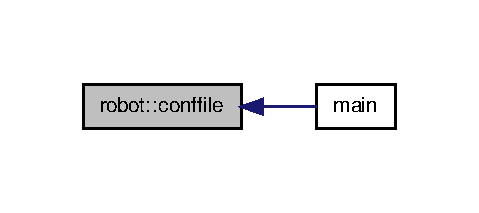
\includegraphics[width=230pt]{classrobot_a35ecdc59dfd28155d9500e0d324f9025_icgraph}
\end{center}
\end{figure}


\hypertarget{classrobot_a18a96780dde613e9bc5504db837cc604}{\index{robot@{robot}!Nav2@{Nav2}}
\index{Nav2@{Nav2}!robot@{robot}}
\subsubsection[{Nav2}]{\setlength{\rightskip}{0pt plus 5cm}int robot\-::\-Nav2 (
\begin{DoxyParamCaption}
\item[{const char $\ast$}]{msg}
\end{DoxyParamCaption}
)}}\label{classrobot_a18a96780dde613e9bc5504db837cc604}


Definition at line 99 of file robot.\-cpp.

\hypertarget{classrobot_a1c7b39f7b02e282220ec8978770eaeee}{\index{robot@{robot}!set\-\_\-configfile@{set\-\_\-configfile}}
\index{set\-\_\-configfile@{set\-\_\-configfile}!robot@{robot}}
\subsubsection[{set\-\_\-configfile}]{\setlength{\rightskip}{0pt plus 5cm}void robot\-::set\-\_\-configfile (
\begin{DoxyParamCaption}
\item[{char $\ast$}]{config}
\end{DoxyParamCaption}
)}}\label{classrobot_a1c7b39f7b02e282220ec8978770eaeee}


Definition at line 62 of file robot.\-cpp.



Here is the caller graph for this function\-:
\nopagebreak
\begin{figure}[H]
\begin{center}
\leavevmode
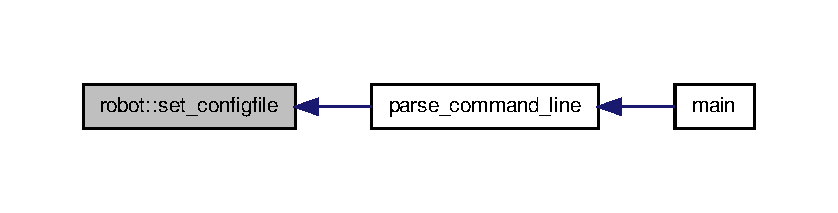
\includegraphics[width=350pt]{classrobot_a1c7b39f7b02e282220ec8978770eaeee_icgraph}
\end{center}
\end{figure}


\hypertarget{classrobot_aeb00885111963664c3b4c0d64db1c42e}{\index{robot@{robot}!set\-\_\-host@{set\-\_\-host}}
\index{set\-\_\-host@{set\-\_\-host}!robot@{robot}}
\subsubsection[{set\-\_\-host}]{\setlength{\rightskip}{0pt plus 5cm}void robot\-::set\-\_\-host (
\begin{DoxyParamCaption}
\item[{char $\ast$}]{host}
\end{DoxyParamCaption}
)}}\label{classrobot_aeb00885111963664c3b4c0d64db1c42e}


Definition at line 50 of file robot.\-cpp.



Here is the caller graph for this function\-:
\nopagebreak
\begin{figure}[H]
\begin{center}
\leavevmode
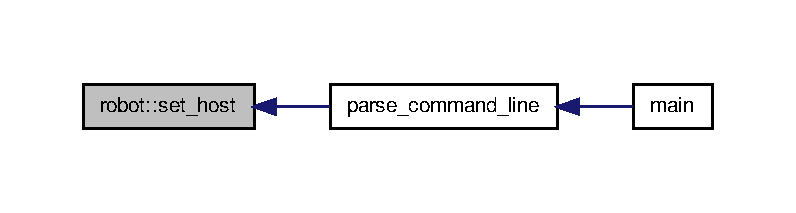
\includegraphics[width=350pt]{classrobot_aeb00885111963664c3b4c0d64db1c42e_icgraph}
\end{center}
\end{figure}


\hypertarget{classrobot_a61dbfda8c9239191e1819e9e9c9a3307}{\index{robot@{robot}!set\-\_\-port@{set\-\_\-port}}
\index{set\-\_\-port@{set\-\_\-port}!robot@{robot}}
\subsubsection[{set\-\_\-port}]{\setlength{\rightskip}{0pt plus 5cm}void robot\-::set\-\_\-port (
\begin{DoxyParamCaption}
\item[{int}]{portno}
\end{DoxyParamCaption}
)}}\label{classrobot_a61dbfda8c9239191e1819e9e9c9a3307}


Definition at line 56 of file robot.\-cpp.



Here is the caller graph for this function\-:
\nopagebreak
\begin{figure}[H]
\begin{center}
\leavevmode
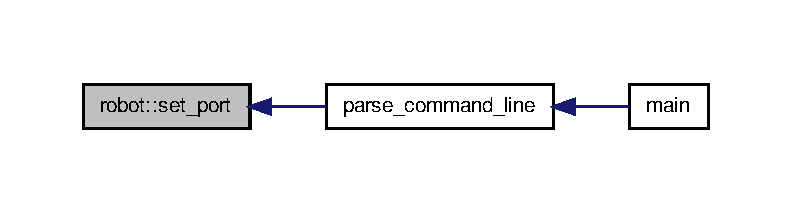
\includegraphics[width=350pt]{classrobot_a61dbfda8c9239191e1819e9e9c9a3307_icgraph}
\end{center}
\end{figure}


\hypertarget{classrobot_a3fe4a564af34323851bc1bcc7481e865}{\index{robot@{robot}!tcp\-\_\-connect@{tcp\-\_\-connect}}
\index{tcp\-\_\-connect@{tcp\-\_\-connect}!robot@{robot}}
\subsubsection[{tcp\-\_\-connect}]{\setlength{\rightskip}{0pt plus 5cm}int robot\-::tcp\-\_\-connect (
\begin{DoxyParamCaption}
{}
\end{DoxyParamCaption}
)}}\label{classrobot_a3fe4a564af34323851bc1bcc7481e865}


Definition at line 74 of file robot.\-cpp.



Here is the call graph for this function\-:
\nopagebreak
\begin{figure}[H]
\begin{center}
\leavevmode
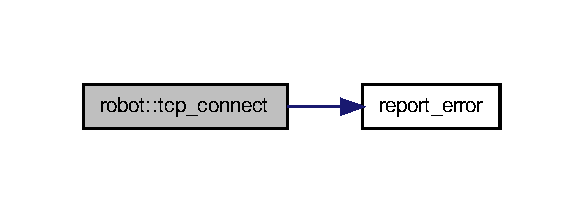
\includegraphics[width=280pt]{classrobot_a3fe4a564af34323851bc1bcc7481e865_cgraph}
\end{center}
\end{figure}


\hypertarget{classrobot_a2d9f6439790b1c73e02878d27826109f}{\index{robot@{robot}!update\-\_\-poshead@{update\-\_\-poshead}}
\index{update\-\_\-poshead@{update\-\_\-poshead}!robot@{robot}}
\subsubsection[{update\-\_\-poshead}]{\setlength{\rightskip}{0pt plus 5cm}void robot\-::update\-\_\-poshead (
\begin{DoxyParamCaption}
{}
\end{DoxyParamCaption}
)}}\label{classrobot_a2d9f6439790b1c73e02878d27826109f}


Definition at line 104 of file robot.\-cpp.



Here is the call graph for this function\-:
\nopagebreak
\begin{figure}[H]
\begin{center}
\leavevmode
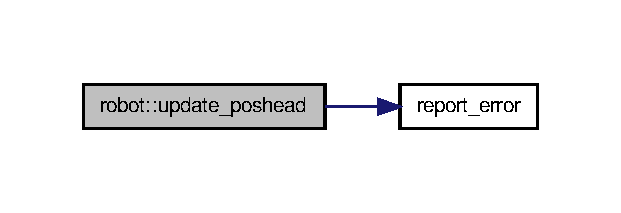
\includegraphics[width=298pt]{classrobot_a2d9f6439790b1c73e02878d27826109f_cgraph}
\end{center}
\end{figure}




The documentation for this class was generated from the following files\-:\begin{DoxyCompactItemize}
\item 
src/\hyperlink{robot_8h}{robot.\-h}\item 
src/\hyperlink{robot_8cpp}{robot.\-cpp}\end{DoxyCompactItemize}

\chapter{File Documentation}
\hypertarget{errhandler_8cpp}{\section{src/errhandler.cpp File Reference}
\label{errhandler_8cpp}\index{src/errhandler.\-cpp@{src/errhandler.\-cpp}}
}
{\ttfamily \#include $<$stdio.\-h$>$}\\*
{\ttfamily \#include $<$stdlib.\-h$>$}\\*
{\ttfamily \#include \char`\"{}error\-\_\-codes.\-h\char`\"{}}\\*
Include dependency graph for errhandler.\-cpp\-:
\nopagebreak
\begin{figure}[H]
\begin{center}
\leavevmode
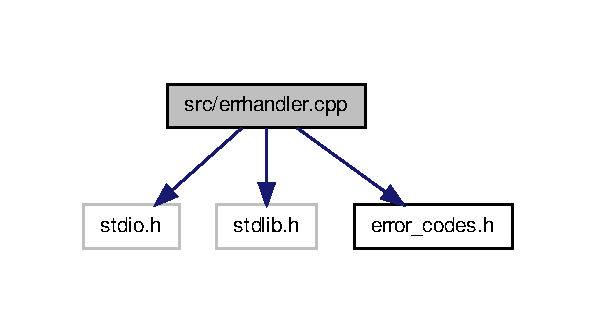
\includegraphics[width=286pt]{errhandler_8cpp__incl}
\end{center}
\end{figure}
\subsection*{Functions}
\begin{DoxyCompactItemize}
\item 
void \hyperlink{errhandler_8cpp_a404519733fecb82a4172f2fc29d511f7}{report\-\_\-error} (const int errno, const char $\ast$notes)
\end{DoxyCompactItemize}


\subsection{Function Documentation}
\hypertarget{errhandler_8cpp_a404519733fecb82a4172f2fc29d511f7}{\index{errhandler.\-cpp@{errhandler.\-cpp}!report\-\_\-error@{report\-\_\-error}}
\index{report\-\_\-error@{report\-\_\-error}!errhandler.cpp@{errhandler.\-cpp}}
\subsubsection[{report\-\_\-error}]{\setlength{\rightskip}{0pt plus 5cm}void report\-\_\-error (
\begin{DoxyParamCaption}
\item[{const int}]{errno, }
\item[{const char $\ast$}]{notes}
\end{DoxyParamCaption}
)}}\label{errhandler_8cpp_a404519733fecb82a4172f2fc29d511f7}


Definition at line 26 of file errhandler.\-cpp.



Here is the caller graph for this function\-:
\nopagebreak
\begin{figure}[H]
\begin{center}
\leavevmode
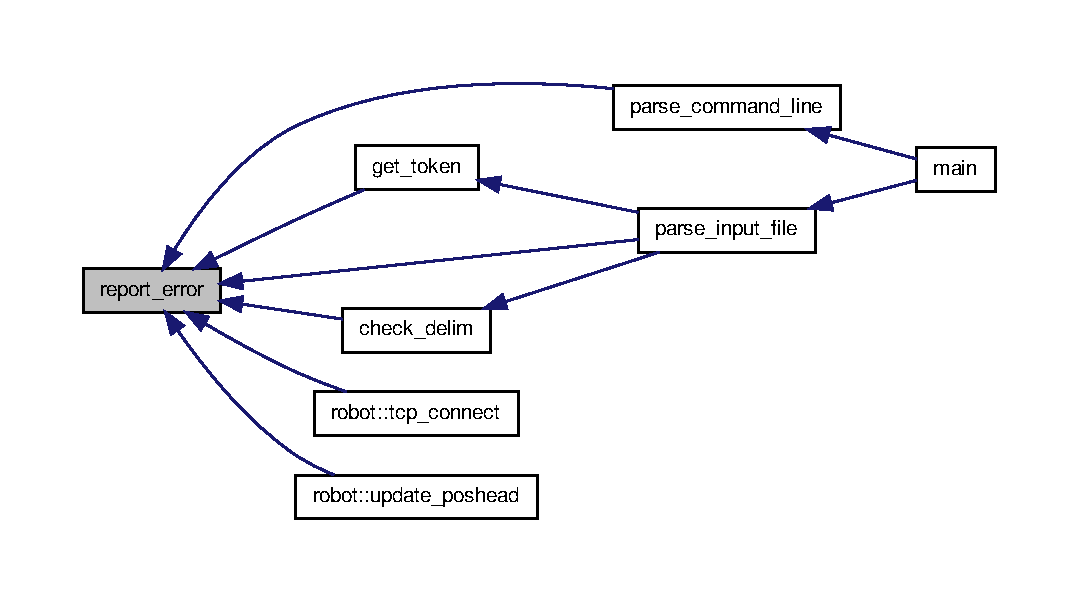
\includegraphics[width=350pt]{errhandler_8cpp_a404519733fecb82a4172f2fc29d511f7_icgraph}
\end{center}
\end{figure}



\hypertarget{errinclude_8h}{\section{src/errinclude.h File Reference}
\label{errinclude_8h}\index{src/errinclude.\-h@{src/errinclude.\-h}}
}
{\ttfamily \#include \char`\"{}error\-\_\-codes.\-h\char`\"{}}\\*
Include dependency graph for errinclude.\-h\-:
\nopagebreak
\begin{figure}[H]
\begin{center}
\leavevmode
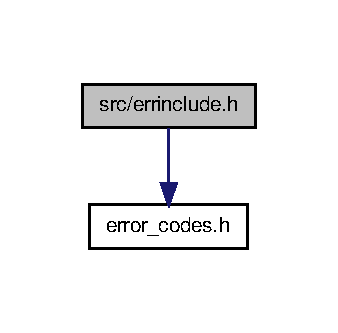
\includegraphics[width=162pt]{errinclude_8h__incl}
\end{center}
\end{figure}
This graph shows which files directly or indirectly include this file\-:
\nopagebreak
\begin{figure}[H]
\begin{center}
\leavevmode
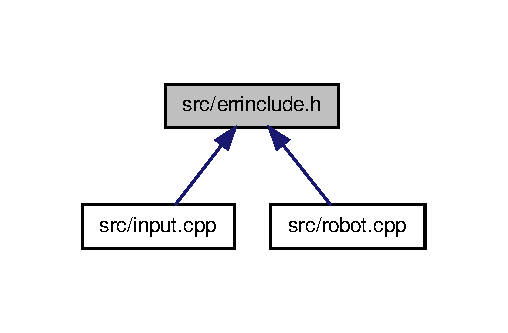
\includegraphics[width=244pt]{errinclude_8h__dep__incl}
\end{center}
\end{figure}
\subsection*{Functions}
\begin{DoxyCompactItemize}
\item 
void \hyperlink{errinclude_8h_adc9eef70042bbef4104764beda1c2f44}{report\-\_\-error} (const int, const char $\ast$)
\end{DoxyCompactItemize}


\subsection{Function Documentation}
\hypertarget{errinclude_8h_adc9eef70042bbef4104764beda1c2f44}{\index{errinclude.\-h@{errinclude.\-h}!report\-\_\-error@{report\-\_\-error}}
\index{report\-\_\-error@{report\-\_\-error}!errinclude.h@{errinclude.\-h}}
\subsubsection[{report\-\_\-error}]{\setlength{\rightskip}{0pt plus 5cm}void report\-\_\-error (
\begin{DoxyParamCaption}
\item[{const int}]{, }
\item[{const char $\ast$}]{}
\end{DoxyParamCaption}
)}}\label{errinclude_8h_adc9eef70042bbef4104764beda1c2f44}


Definition at line 26 of file errhandler.\-cpp.



Here is the caller graph for this function\-:
\nopagebreak
\begin{figure}[H]
\begin{center}
\leavevmode
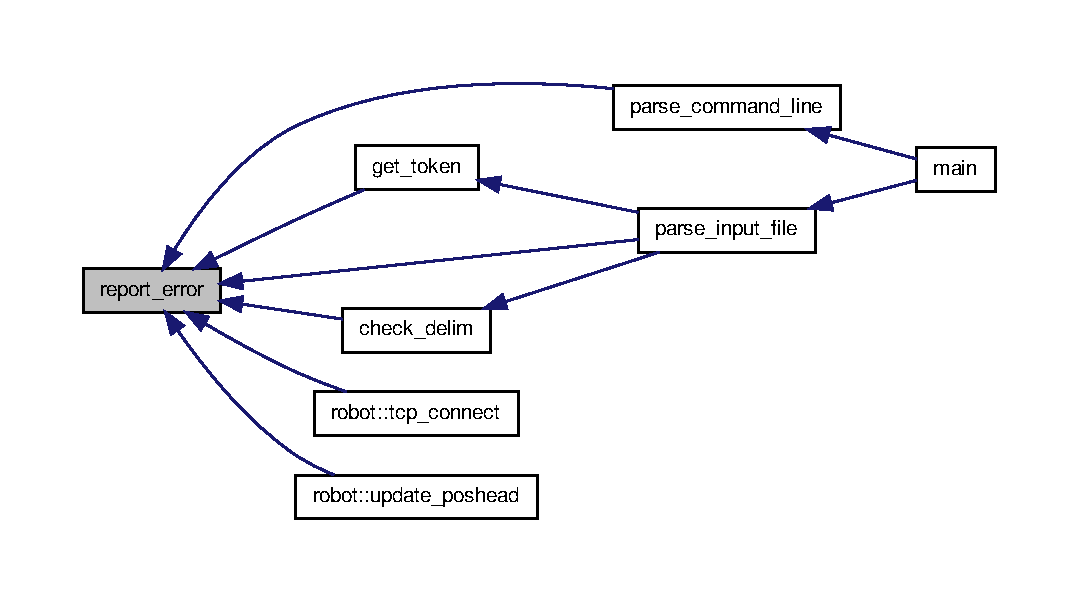
\includegraphics[width=350pt]{errinclude_8h_adc9eef70042bbef4104764beda1c2f44_icgraph}
\end{center}
\end{figure}



\hypertarget{error__codes_8h}{\section{src/error\-\_\-codes.h File Reference}
\label{error__codes_8h}\index{src/error\-\_\-codes.\-h@{src/error\-\_\-codes.\-h}}
}
This graph shows which files directly or indirectly include this file\-:
\nopagebreak
\begin{figure}[H]
\begin{center}
\leavevmode
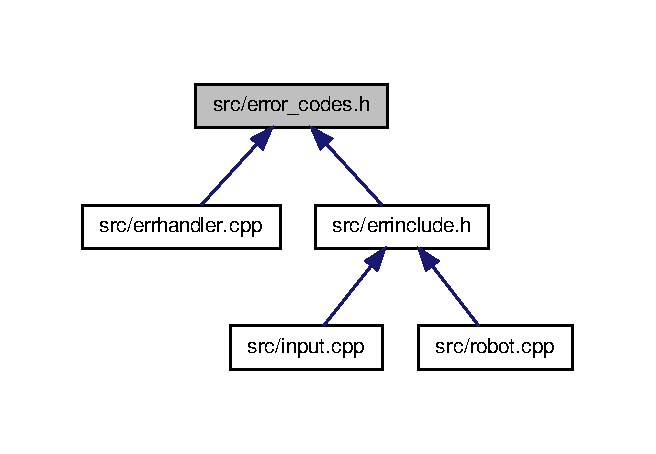
\includegraphics[width=315pt]{error__codes_8h__dep__incl}
\end{center}
\end{figure}
\subsection*{Macros}
\begin{DoxyCompactItemize}
\item 
\#define \hyperlink{error__codes_8h_a6aa5eeeca15a6c21bd63d80c60a2c7f0}{S\-O\-C\-K\-\_\-\-C\-A\-N\-N\-O\-T\-\_\-\-C\-R\-E\-A\-T\-E\-\_\-\-S\-O\-C\-K}~0x11
\item 
\#define \hyperlink{error__codes_8h_a4aa3d98de652b4accad3d99e6ee826f8}{S\-O\-C\-K\-\_\-\-C\-A\-N\-N\-O\-T\-\_\-\-C\-O\-N\-N\-E\-C\-T}~0x12
\item 
\#define \hyperlink{error__codes_8h_aff3a3001a999a493dfbe93601173e126}{C\-L\-\_\-\-N\-O\-\_\-\-A\-R\-G}~0x13
\item 
\#define \hyperlink{error__codes_8h_a4663dd5c312670e4f72c360151b9223e}{C\-L\-\_\-\-I\-N\-V\-A\-L\-I\-D\-\_\-\-O\-P\-T}~0x14
\item 
\#define \hyperlink{error__codes_8h_a0d5d6725964b19dbb21fcaa261523d61}{C\-L\-\_\-\-U\-N\-K\-O\-W\-N\-\_\-\-O\-P\-T\-\_\-\-C\-H\-A\-R}~0x15
\item 
\#define \hyperlink{error__codes_8h_a9c21f3d072c0975ae6cb4535086a0b2a}{S\-O\-C\-K\-\_\-\-R\-E\-A\-D\-\_\-\-E\-R\-R\-O\-R}~0x16
\item 
\#define \hyperlink{error__codes_8h_a5ffe7acc9e73f89dc367287028c456cd}{S\-O\-C\-K\-\_\-\-W\-R\-I\-T\-E\-\_\-\-E\-R\-R\-O\-R}~0x17
\item 
\#define \hyperlink{error__codes_8h_aa876a310c9ab41cb2cf2536cdd8aa59d}{C\-A\-N\-N\-O\-T\-\_\-\-O\-P\-E\-N\-\_\-\-I\-N\-F\-I\-L\-E}~0x18
\item 
\#define \hyperlink{error__codes_8h_aad77768f0bb82f310977558ce9e37e9c}{C\-A\-N\-N\-O\-T\-\_\-\-R\-E\-A\-D\-\_\-\-I\-N\-F\-I\-L\-E}~0x19
\item 
\#define \hyperlink{error__codes_8h_ac3b27c4697cbbfc6352cd7cfc440bf96}{I\-N\-V\-A\-L\-I\-D\-\_\-\-I\-N\-P\-U\-T\-\_\-\-F\-I\-L\-E\-\_\-\-S\-Y\-N\-T\-A\-X}~0x1\-A
\item 
\#define \hyperlink{error__codes_8h_a025b98311531fefa3c67a52ca21e7c89}{R\-E\-C\-O\-V\-E\-R\-A\-B\-L\-E\-\_\-\-I\-N\-P\-U\-T\-\_\-\-F\-I\-L\-E\-\_\-\-S\-Y\-N\-T\-A\-X}~0x1\-B
\item 
\#define \hyperlink{error__codes_8h_aeea5cde21b8e63f1f873f6c665743f2b}{F\-A\-T\-A\-L\-\_\-\-I\-N\-P\-U\-T\-\_\-\-F\-I\-L\-E\-\_\-\-S\-Y\-N\-T\-A\-X}~0x1\-C
\end{DoxyCompactItemize}


\subsection{Macro Definition Documentation}
\hypertarget{error__codes_8h_aa876a310c9ab41cb2cf2536cdd8aa59d}{\index{error\-\_\-codes.\-h@{error\-\_\-codes.\-h}!C\-A\-N\-N\-O\-T\-\_\-\-O\-P\-E\-N\-\_\-\-I\-N\-F\-I\-L\-E@{C\-A\-N\-N\-O\-T\-\_\-\-O\-P\-E\-N\-\_\-\-I\-N\-F\-I\-L\-E}}
\index{C\-A\-N\-N\-O\-T\-\_\-\-O\-P\-E\-N\-\_\-\-I\-N\-F\-I\-L\-E@{C\-A\-N\-N\-O\-T\-\_\-\-O\-P\-E\-N\-\_\-\-I\-N\-F\-I\-L\-E}!error_codes.h@{error\-\_\-codes.\-h}}
\subsubsection[{C\-A\-N\-N\-O\-T\-\_\-\-O\-P\-E\-N\-\_\-\-I\-N\-F\-I\-L\-E}]{\setlength{\rightskip}{0pt plus 5cm}\#define C\-A\-N\-N\-O\-T\-\_\-\-O\-P\-E\-N\-\_\-\-I\-N\-F\-I\-L\-E~0x18}}\label{error__codes_8h_aa876a310c9ab41cb2cf2536cdd8aa59d}


Definition at line 31 of file error\-\_\-codes.\-h.

\hypertarget{error__codes_8h_aad77768f0bb82f310977558ce9e37e9c}{\index{error\-\_\-codes.\-h@{error\-\_\-codes.\-h}!C\-A\-N\-N\-O\-T\-\_\-\-R\-E\-A\-D\-\_\-\-I\-N\-F\-I\-L\-E@{C\-A\-N\-N\-O\-T\-\_\-\-R\-E\-A\-D\-\_\-\-I\-N\-F\-I\-L\-E}}
\index{C\-A\-N\-N\-O\-T\-\_\-\-R\-E\-A\-D\-\_\-\-I\-N\-F\-I\-L\-E@{C\-A\-N\-N\-O\-T\-\_\-\-R\-E\-A\-D\-\_\-\-I\-N\-F\-I\-L\-E}!error_codes.h@{error\-\_\-codes.\-h}}
\subsubsection[{C\-A\-N\-N\-O\-T\-\_\-\-R\-E\-A\-D\-\_\-\-I\-N\-F\-I\-L\-E}]{\setlength{\rightskip}{0pt plus 5cm}\#define C\-A\-N\-N\-O\-T\-\_\-\-R\-E\-A\-D\-\_\-\-I\-N\-F\-I\-L\-E~0x19}}\label{error__codes_8h_aad77768f0bb82f310977558ce9e37e9c}


Definition at line 32 of file error\-\_\-codes.\-h.

\hypertarget{error__codes_8h_a4663dd5c312670e4f72c360151b9223e}{\index{error\-\_\-codes.\-h@{error\-\_\-codes.\-h}!C\-L\-\_\-\-I\-N\-V\-A\-L\-I\-D\-\_\-\-O\-P\-T@{C\-L\-\_\-\-I\-N\-V\-A\-L\-I\-D\-\_\-\-O\-P\-T}}
\index{C\-L\-\_\-\-I\-N\-V\-A\-L\-I\-D\-\_\-\-O\-P\-T@{C\-L\-\_\-\-I\-N\-V\-A\-L\-I\-D\-\_\-\-O\-P\-T}!error_codes.h@{error\-\_\-codes.\-h}}
\subsubsection[{C\-L\-\_\-\-I\-N\-V\-A\-L\-I\-D\-\_\-\-O\-P\-T}]{\setlength{\rightskip}{0pt plus 5cm}\#define C\-L\-\_\-\-I\-N\-V\-A\-L\-I\-D\-\_\-\-O\-P\-T~0x14}}\label{error__codes_8h_a4663dd5c312670e4f72c360151b9223e}


Definition at line 27 of file error\-\_\-codes.\-h.

\hypertarget{error__codes_8h_aff3a3001a999a493dfbe93601173e126}{\index{error\-\_\-codes.\-h@{error\-\_\-codes.\-h}!C\-L\-\_\-\-N\-O\-\_\-\-A\-R\-G@{C\-L\-\_\-\-N\-O\-\_\-\-A\-R\-G}}
\index{C\-L\-\_\-\-N\-O\-\_\-\-A\-R\-G@{C\-L\-\_\-\-N\-O\-\_\-\-A\-R\-G}!error_codes.h@{error\-\_\-codes.\-h}}
\subsubsection[{C\-L\-\_\-\-N\-O\-\_\-\-A\-R\-G}]{\setlength{\rightskip}{0pt plus 5cm}\#define C\-L\-\_\-\-N\-O\-\_\-\-A\-R\-G~0x13}}\label{error__codes_8h_aff3a3001a999a493dfbe93601173e126}


Definition at line 26 of file error\-\_\-codes.\-h.

\hypertarget{error__codes_8h_a0d5d6725964b19dbb21fcaa261523d61}{\index{error\-\_\-codes.\-h@{error\-\_\-codes.\-h}!C\-L\-\_\-\-U\-N\-K\-O\-W\-N\-\_\-\-O\-P\-T\-\_\-\-C\-H\-A\-R@{C\-L\-\_\-\-U\-N\-K\-O\-W\-N\-\_\-\-O\-P\-T\-\_\-\-C\-H\-A\-R}}
\index{C\-L\-\_\-\-U\-N\-K\-O\-W\-N\-\_\-\-O\-P\-T\-\_\-\-C\-H\-A\-R@{C\-L\-\_\-\-U\-N\-K\-O\-W\-N\-\_\-\-O\-P\-T\-\_\-\-C\-H\-A\-R}!error_codes.h@{error\-\_\-codes.\-h}}
\subsubsection[{C\-L\-\_\-\-U\-N\-K\-O\-W\-N\-\_\-\-O\-P\-T\-\_\-\-C\-H\-A\-R}]{\setlength{\rightskip}{0pt plus 5cm}\#define C\-L\-\_\-\-U\-N\-K\-O\-W\-N\-\_\-\-O\-P\-T\-\_\-\-C\-H\-A\-R~0x15}}\label{error__codes_8h_a0d5d6725964b19dbb21fcaa261523d61}


Definition at line 28 of file error\-\_\-codes.\-h.

\hypertarget{error__codes_8h_aeea5cde21b8e63f1f873f6c665743f2b}{\index{error\-\_\-codes.\-h@{error\-\_\-codes.\-h}!F\-A\-T\-A\-L\-\_\-\-I\-N\-P\-U\-T\-\_\-\-F\-I\-L\-E\-\_\-\-S\-Y\-N\-T\-A\-X@{F\-A\-T\-A\-L\-\_\-\-I\-N\-P\-U\-T\-\_\-\-F\-I\-L\-E\-\_\-\-S\-Y\-N\-T\-A\-X}}
\index{F\-A\-T\-A\-L\-\_\-\-I\-N\-P\-U\-T\-\_\-\-F\-I\-L\-E\-\_\-\-S\-Y\-N\-T\-A\-X@{F\-A\-T\-A\-L\-\_\-\-I\-N\-P\-U\-T\-\_\-\-F\-I\-L\-E\-\_\-\-S\-Y\-N\-T\-A\-X}!error_codes.h@{error\-\_\-codes.\-h}}
\subsubsection[{F\-A\-T\-A\-L\-\_\-\-I\-N\-P\-U\-T\-\_\-\-F\-I\-L\-E\-\_\-\-S\-Y\-N\-T\-A\-X}]{\setlength{\rightskip}{0pt plus 5cm}\#define F\-A\-T\-A\-L\-\_\-\-I\-N\-P\-U\-T\-\_\-\-F\-I\-L\-E\-\_\-\-S\-Y\-N\-T\-A\-X~0x1\-C}}\label{error__codes_8h_aeea5cde21b8e63f1f873f6c665743f2b}


Definition at line 35 of file error\-\_\-codes.\-h.

\hypertarget{error__codes_8h_ac3b27c4697cbbfc6352cd7cfc440bf96}{\index{error\-\_\-codes.\-h@{error\-\_\-codes.\-h}!I\-N\-V\-A\-L\-I\-D\-\_\-\-I\-N\-P\-U\-T\-\_\-\-F\-I\-L\-E\-\_\-\-S\-Y\-N\-T\-A\-X@{I\-N\-V\-A\-L\-I\-D\-\_\-\-I\-N\-P\-U\-T\-\_\-\-F\-I\-L\-E\-\_\-\-S\-Y\-N\-T\-A\-X}}
\index{I\-N\-V\-A\-L\-I\-D\-\_\-\-I\-N\-P\-U\-T\-\_\-\-F\-I\-L\-E\-\_\-\-S\-Y\-N\-T\-A\-X@{I\-N\-V\-A\-L\-I\-D\-\_\-\-I\-N\-P\-U\-T\-\_\-\-F\-I\-L\-E\-\_\-\-S\-Y\-N\-T\-A\-X}!error_codes.h@{error\-\_\-codes.\-h}}
\subsubsection[{I\-N\-V\-A\-L\-I\-D\-\_\-\-I\-N\-P\-U\-T\-\_\-\-F\-I\-L\-E\-\_\-\-S\-Y\-N\-T\-A\-X}]{\setlength{\rightskip}{0pt plus 5cm}\#define I\-N\-V\-A\-L\-I\-D\-\_\-\-I\-N\-P\-U\-T\-\_\-\-F\-I\-L\-E\-\_\-\-S\-Y\-N\-T\-A\-X~0x1\-A}}\label{error__codes_8h_ac3b27c4697cbbfc6352cd7cfc440bf96}


Definition at line 33 of file error\-\_\-codes.\-h.

\hypertarget{error__codes_8h_a025b98311531fefa3c67a52ca21e7c89}{\index{error\-\_\-codes.\-h@{error\-\_\-codes.\-h}!R\-E\-C\-O\-V\-E\-R\-A\-B\-L\-E\-\_\-\-I\-N\-P\-U\-T\-\_\-\-F\-I\-L\-E\-\_\-\-S\-Y\-N\-T\-A\-X@{R\-E\-C\-O\-V\-E\-R\-A\-B\-L\-E\-\_\-\-I\-N\-P\-U\-T\-\_\-\-F\-I\-L\-E\-\_\-\-S\-Y\-N\-T\-A\-X}}
\index{R\-E\-C\-O\-V\-E\-R\-A\-B\-L\-E\-\_\-\-I\-N\-P\-U\-T\-\_\-\-F\-I\-L\-E\-\_\-\-S\-Y\-N\-T\-A\-X@{R\-E\-C\-O\-V\-E\-R\-A\-B\-L\-E\-\_\-\-I\-N\-P\-U\-T\-\_\-\-F\-I\-L\-E\-\_\-\-S\-Y\-N\-T\-A\-X}!error_codes.h@{error\-\_\-codes.\-h}}
\subsubsection[{R\-E\-C\-O\-V\-E\-R\-A\-B\-L\-E\-\_\-\-I\-N\-P\-U\-T\-\_\-\-F\-I\-L\-E\-\_\-\-S\-Y\-N\-T\-A\-X}]{\setlength{\rightskip}{0pt plus 5cm}\#define R\-E\-C\-O\-V\-E\-R\-A\-B\-L\-E\-\_\-\-I\-N\-P\-U\-T\-\_\-\-F\-I\-L\-E\-\_\-\-S\-Y\-N\-T\-A\-X~0x1\-B}}\label{error__codes_8h_a025b98311531fefa3c67a52ca21e7c89}


Definition at line 34 of file error\-\_\-codes.\-h.

\hypertarget{error__codes_8h_a4aa3d98de652b4accad3d99e6ee826f8}{\index{error\-\_\-codes.\-h@{error\-\_\-codes.\-h}!S\-O\-C\-K\-\_\-\-C\-A\-N\-N\-O\-T\-\_\-\-C\-O\-N\-N\-E\-C\-T@{S\-O\-C\-K\-\_\-\-C\-A\-N\-N\-O\-T\-\_\-\-C\-O\-N\-N\-E\-C\-T}}
\index{S\-O\-C\-K\-\_\-\-C\-A\-N\-N\-O\-T\-\_\-\-C\-O\-N\-N\-E\-C\-T@{S\-O\-C\-K\-\_\-\-C\-A\-N\-N\-O\-T\-\_\-\-C\-O\-N\-N\-E\-C\-T}!error_codes.h@{error\-\_\-codes.\-h}}
\subsubsection[{S\-O\-C\-K\-\_\-\-C\-A\-N\-N\-O\-T\-\_\-\-C\-O\-N\-N\-E\-C\-T}]{\setlength{\rightskip}{0pt plus 5cm}\#define S\-O\-C\-K\-\_\-\-C\-A\-N\-N\-O\-T\-\_\-\-C\-O\-N\-N\-E\-C\-T~0x12}}\label{error__codes_8h_a4aa3d98de652b4accad3d99e6ee826f8}


Definition at line 25 of file error\-\_\-codes.\-h.

\hypertarget{error__codes_8h_a6aa5eeeca15a6c21bd63d80c60a2c7f0}{\index{error\-\_\-codes.\-h@{error\-\_\-codes.\-h}!S\-O\-C\-K\-\_\-\-C\-A\-N\-N\-O\-T\-\_\-\-C\-R\-E\-A\-T\-E\-\_\-\-S\-O\-C\-K@{S\-O\-C\-K\-\_\-\-C\-A\-N\-N\-O\-T\-\_\-\-C\-R\-E\-A\-T\-E\-\_\-\-S\-O\-C\-K}}
\index{S\-O\-C\-K\-\_\-\-C\-A\-N\-N\-O\-T\-\_\-\-C\-R\-E\-A\-T\-E\-\_\-\-S\-O\-C\-K@{S\-O\-C\-K\-\_\-\-C\-A\-N\-N\-O\-T\-\_\-\-C\-R\-E\-A\-T\-E\-\_\-\-S\-O\-C\-K}!error_codes.h@{error\-\_\-codes.\-h}}
\subsubsection[{S\-O\-C\-K\-\_\-\-C\-A\-N\-N\-O\-T\-\_\-\-C\-R\-E\-A\-T\-E\-\_\-\-S\-O\-C\-K}]{\setlength{\rightskip}{0pt plus 5cm}\#define S\-O\-C\-K\-\_\-\-C\-A\-N\-N\-O\-T\-\_\-\-C\-R\-E\-A\-T\-E\-\_\-\-S\-O\-C\-K~0x11}}\label{error__codes_8h_a6aa5eeeca15a6c21bd63d80c60a2c7f0}


Definition at line 24 of file error\-\_\-codes.\-h.

\hypertarget{error__codes_8h_a9c21f3d072c0975ae6cb4535086a0b2a}{\index{error\-\_\-codes.\-h@{error\-\_\-codes.\-h}!S\-O\-C\-K\-\_\-\-R\-E\-A\-D\-\_\-\-E\-R\-R\-O\-R@{S\-O\-C\-K\-\_\-\-R\-E\-A\-D\-\_\-\-E\-R\-R\-O\-R}}
\index{S\-O\-C\-K\-\_\-\-R\-E\-A\-D\-\_\-\-E\-R\-R\-O\-R@{S\-O\-C\-K\-\_\-\-R\-E\-A\-D\-\_\-\-E\-R\-R\-O\-R}!error_codes.h@{error\-\_\-codes.\-h}}
\subsubsection[{S\-O\-C\-K\-\_\-\-R\-E\-A\-D\-\_\-\-E\-R\-R\-O\-R}]{\setlength{\rightskip}{0pt plus 5cm}\#define S\-O\-C\-K\-\_\-\-R\-E\-A\-D\-\_\-\-E\-R\-R\-O\-R~0x16}}\label{error__codes_8h_a9c21f3d072c0975ae6cb4535086a0b2a}


Definition at line 29 of file error\-\_\-codes.\-h.

\hypertarget{error__codes_8h_a5ffe7acc9e73f89dc367287028c456cd}{\index{error\-\_\-codes.\-h@{error\-\_\-codes.\-h}!S\-O\-C\-K\-\_\-\-W\-R\-I\-T\-E\-\_\-\-E\-R\-R\-O\-R@{S\-O\-C\-K\-\_\-\-W\-R\-I\-T\-E\-\_\-\-E\-R\-R\-O\-R}}
\index{S\-O\-C\-K\-\_\-\-W\-R\-I\-T\-E\-\_\-\-E\-R\-R\-O\-R@{S\-O\-C\-K\-\_\-\-W\-R\-I\-T\-E\-\_\-\-E\-R\-R\-O\-R}!error_codes.h@{error\-\_\-codes.\-h}}
\subsubsection[{S\-O\-C\-K\-\_\-\-W\-R\-I\-T\-E\-\_\-\-E\-R\-R\-O\-R}]{\setlength{\rightskip}{0pt plus 5cm}\#define S\-O\-C\-K\-\_\-\-W\-R\-I\-T\-E\-\_\-\-E\-R\-R\-O\-R~0x17}}\label{error__codes_8h_a5ffe7acc9e73f89dc367287028c456cd}


Definition at line 30 of file error\-\_\-codes.\-h.


\hypertarget{input_8cpp}{\section{src/input.cpp File Reference}
\label{input_8cpp}\index{src/input.\-cpp@{src/input.\-cpp}}
}
{\ttfamily \#include $<$stdio.\-h$>$}\\*
{\ttfamily \#include $<$stdlib.\-h$>$}\\*
{\ttfamily \#include $<$unistd.\-h$>$}\\*
{\ttfamily \#include $<$ctype.\-h$>$}\\*
{\ttfamily \#include $<$string.\-h$>$}\\*
{\ttfamily \#include $<$vector$>$}\\*
{\ttfamily \#include \char`\"{}errinclude.\-h\char`\"{}}\\*
{\ttfamily \#include \char`\"{}robot.\-h\char`\"{}}\\*
{\ttfamily \#include \char`\"{}nmpc.\-h\char`\"{}}\\*
Include dependency graph for input.\-cpp\-:
\nopagebreak
\begin{figure}[H]
\begin{center}
\leavevmode
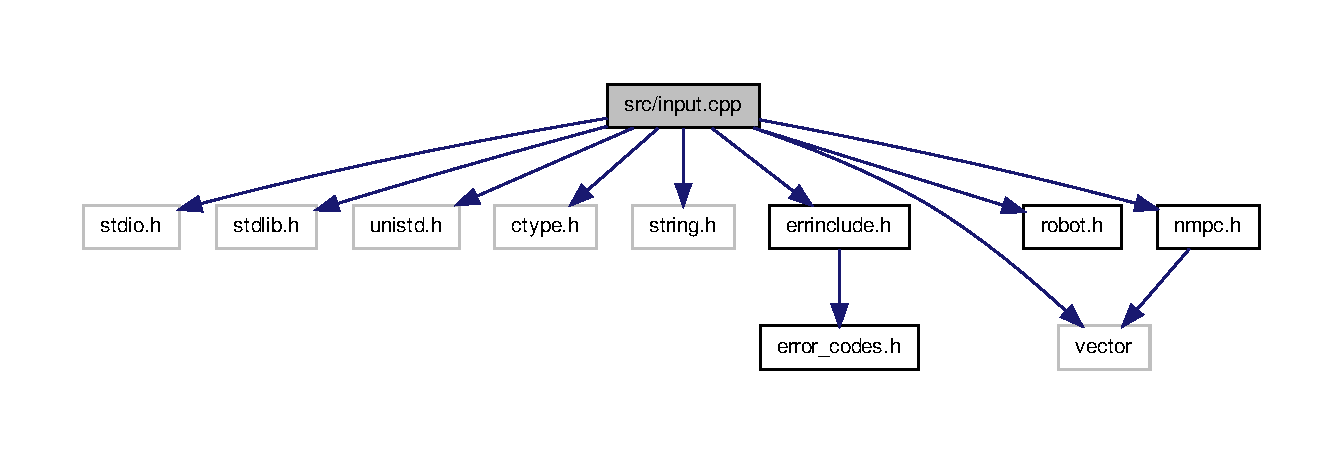
\includegraphics[width=350pt]{input_8cpp__incl}
\end{center}
\end{figure}
\subsection*{Functions}
\begin{DoxyCompactItemize}
\item 
void \hyperlink{input_8cpp_ad19a84e6b6de562e42e80c4ba3a6be88}{parse\-\_\-command\-\_\-line} (int argc, char $\ast$$\ast$argv, \hyperlink{classrobot}{robot} $\ast$vme)
\item 
void \hyperlink{input_8cpp_ac3a302ba089e2df4c2cfb6706c01199b}{get\-\_\-token} (F\-I\-L\-E $\ast$fd, char $\ast$buffer, char $\ast$lastdelim, int $\ast$lineno)
\item 
void \hyperlink{input_8cpp_afc5703718754700cdc592ee59818ea16}{check\-\_\-delim} (char lastdelim, char expected\-\_\-delim, int lineno)
\item 
void \hyperlink{input_8cpp_ad53113827b4fe0ab385a3b0f0b665eaf}{parse\-\_\-input\-\_\-file} (\hyperlink{nmpc_8h_a071459b3a1fa3748660f7de5d6ab38d0}{nmpc} \&controller, const char $\ast$infile)
\end{DoxyCompactItemize}


\subsection{Function Documentation}
\hypertarget{input_8cpp_afc5703718754700cdc592ee59818ea16}{\index{input.\-cpp@{input.\-cpp}!check\-\_\-delim@{check\-\_\-delim}}
\index{check\-\_\-delim@{check\-\_\-delim}!input.cpp@{input.\-cpp}}
\subsubsection[{check\-\_\-delim}]{\setlength{\rightskip}{0pt plus 5cm}void check\-\_\-delim (
\begin{DoxyParamCaption}
\item[{char}]{lastdelim, }
\item[{char}]{expected\-\_\-delim, }
\item[{int}]{lineno}
\end{DoxyParamCaption}
)}}\label{input_8cpp_afc5703718754700cdc592ee59818ea16}


Definition at line 197 of file input.\-cpp.



Here is the call graph for this function\-:
\nopagebreak
\begin{figure}[H]
\begin{center}
\leavevmode
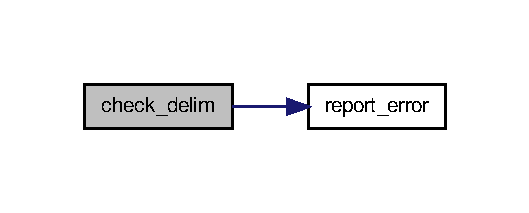
\includegraphics[width=254pt]{input_8cpp_afc5703718754700cdc592ee59818ea16_cgraph}
\end{center}
\end{figure}




Here is the caller graph for this function\-:
\nopagebreak
\begin{figure}[H]
\begin{center}
\leavevmode
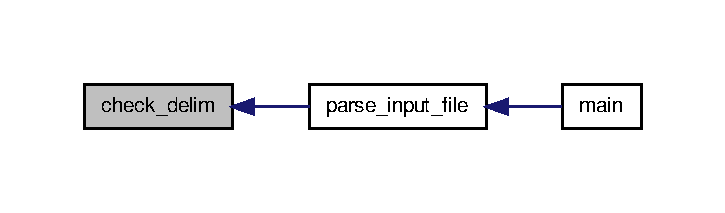
\includegraphics[width=348pt]{input_8cpp_afc5703718754700cdc592ee59818ea16_icgraph}
\end{center}
\end{figure}


\hypertarget{input_8cpp_ac3a302ba089e2df4c2cfb6706c01199b}{\index{input.\-cpp@{input.\-cpp}!get\-\_\-token@{get\-\_\-token}}
\index{get\-\_\-token@{get\-\_\-token}!input.cpp@{input.\-cpp}}
\subsubsection[{get\-\_\-token}]{\setlength{\rightskip}{0pt plus 5cm}void get\-\_\-token (
\begin{DoxyParamCaption}
\item[{F\-I\-L\-E $\ast$}]{fd, }
\item[{char $\ast$}]{buffer, }
\item[{char $\ast$}]{lastdelim, }
\item[{int $\ast$}]{lineno}
\end{DoxyParamCaption}
)}}\label{input_8cpp_ac3a302ba089e2df4c2cfb6706c01199b}


Definition at line 79 of file input.\-cpp.



Here is the call graph for this function\-:
\nopagebreak
\begin{figure}[H]
\begin{center}
\leavevmode
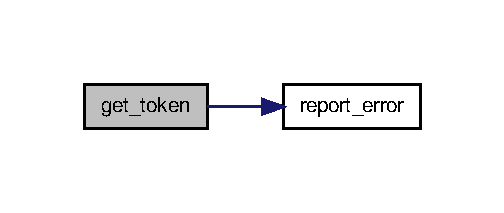
\includegraphics[width=242pt]{input_8cpp_ac3a302ba089e2df4c2cfb6706c01199b_cgraph}
\end{center}
\end{figure}




Here is the caller graph for this function\-:
\nopagebreak
\begin{figure}[H]
\begin{center}
\leavevmode
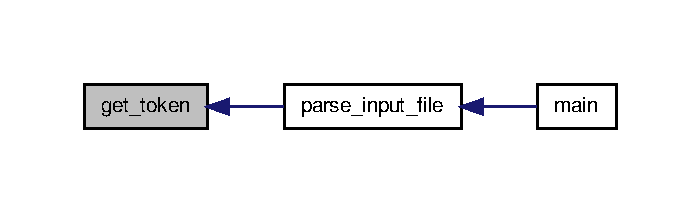
\includegraphics[width=336pt]{input_8cpp_ac3a302ba089e2df4c2cfb6706c01199b_icgraph}
\end{center}
\end{figure}


\hypertarget{input_8cpp_ad19a84e6b6de562e42e80c4ba3a6be88}{\index{input.\-cpp@{input.\-cpp}!parse\-\_\-command\-\_\-line@{parse\-\_\-command\-\_\-line}}
\index{parse\-\_\-command\-\_\-line@{parse\-\_\-command\-\_\-line}!input.cpp@{input.\-cpp}}
\subsubsection[{parse\-\_\-command\-\_\-line}]{\setlength{\rightskip}{0pt plus 5cm}void parse\-\_\-command\-\_\-line (
\begin{DoxyParamCaption}
\item[{int}]{argc, }
\item[{char $\ast$$\ast$}]{argv, }
\item[{{\bf robot} $\ast$}]{vme}
\end{DoxyParamCaption}
)}}\label{input_8cpp_ad19a84e6b6de562e42e80c4ba3a6be88}


Definition at line 32 of file input.\-cpp.



Here is the call graph for this function\-:
\nopagebreak
\begin{figure}[H]
\begin{center}
\leavevmode
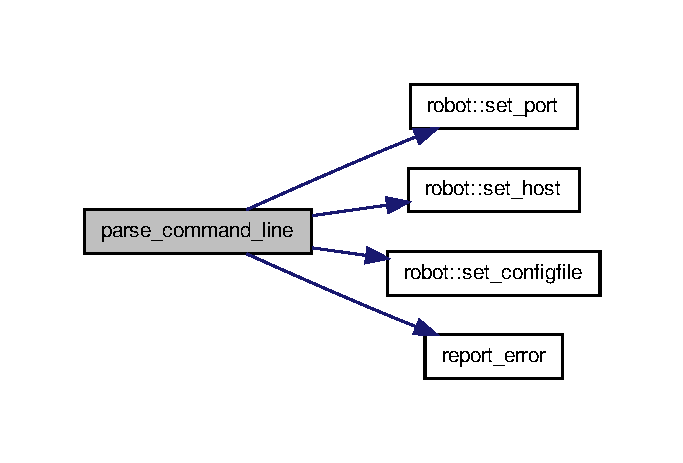
\includegraphics[width=328pt]{input_8cpp_ad19a84e6b6de562e42e80c4ba3a6be88_cgraph}
\end{center}
\end{figure}




Here is the caller graph for this function\-:
\nopagebreak
\begin{figure}[H]
\begin{center}
\leavevmode
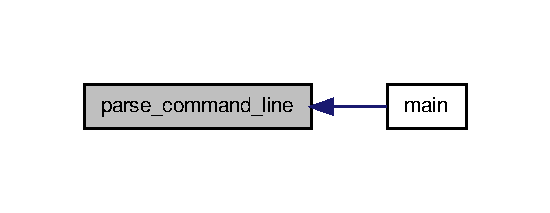
\includegraphics[width=264pt]{input_8cpp_ad19a84e6b6de562e42e80c4ba3a6be88_icgraph}
\end{center}
\end{figure}


\hypertarget{input_8cpp_ad53113827b4fe0ab385a3b0f0b665eaf}{\index{input.\-cpp@{input.\-cpp}!parse\-\_\-input\-\_\-file@{parse\-\_\-input\-\_\-file}}
\index{parse\-\_\-input\-\_\-file@{parse\-\_\-input\-\_\-file}!input.cpp@{input.\-cpp}}
\subsubsection[{parse\-\_\-input\-\_\-file}]{\setlength{\rightskip}{0pt plus 5cm}void parse\-\_\-input\-\_\-file (
\begin{DoxyParamCaption}
\item[{{\bf nmpc} \&}]{controller, }
\item[{const char $\ast$}]{infile}
\end{DoxyParamCaption}
)}}\label{input_8cpp_ad53113827b4fe0ab385a3b0f0b665eaf}


Definition at line 215 of file input.\-cpp.



Here is the call graph for this function\-:
\nopagebreak
\begin{figure}[H]
\begin{center}
\leavevmode
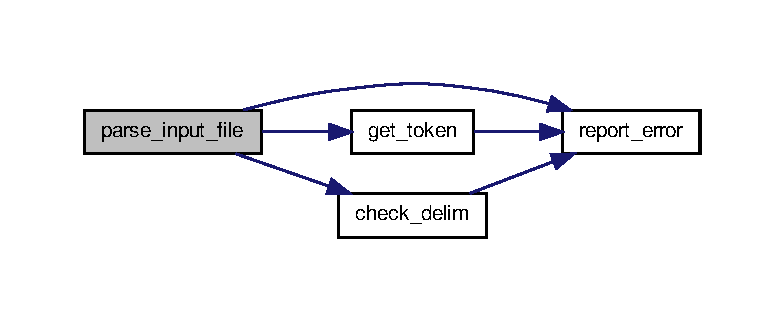
\includegraphics[width=350pt]{input_8cpp_ad53113827b4fe0ab385a3b0f0b665eaf_cgraph}
\end{center}
\end{figure}




Here is the caller graph for this function\-:
\nopagebreak
\begin{figure}[H]
\begin{center}
\leavevmode
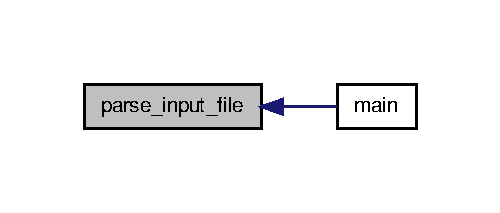
\includegraphics[width=240pt]{input_8cpp_ad53113827b4fe0ab385a3b0f0b665eaf_icgraph}
\end{center}
\end{figure}



\hypertarget{nmpc_8h}{\section{src/nmpc.h File Reference}
\label{nmpc_8h}\index{src/nmpc.\-h@{src/nmpc.\-h}}
}
{\ttfamily \#include $<$vector$>$}\\*
Include dependency graph for nmpc.\-h\-:
\nopagebreak
\begin{figure}[H]
\begin{center}
\leavevmode
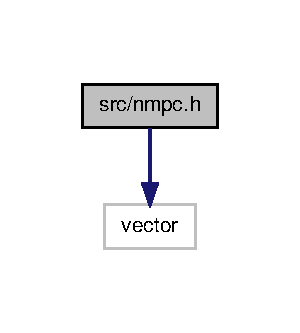
\includegraphics[width=144pt]{nmpc_8h__incl}
\end{center}
\end{figure}
This graph shows which files directly or indirectly include this file\-:
\nopagebreak
\begin{figure}[H]
\begin{center}
\leavevmode
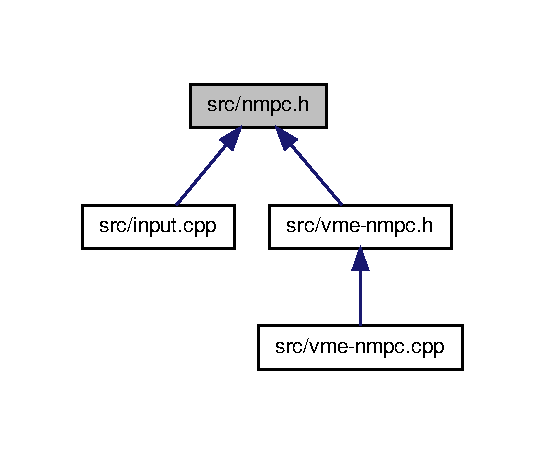
\includegraphics[width=262pt]{nmpc_8h__dep__incl}
\end{center}
\end{figure}
\subsection*{Classes}
\begin{DoxyCompactItemize}
\item 
struct \hyperlink{structnmpc__tag}{nmpc\-\_\-tag}
\end{DoxyCompactItemize}
\subsection*{Typedefs}
\begin{DoxyCompactItemize}
\item 
typedef struct \hyperlink{structnmpc__tag}{nmpc\-\_\-tag} \hyperlink{nmpc_8h_a071459b3a1fa3748660f7de5d6ab38d0}{nmpc}
\end{DoxyCompactItemize}


\subsection{Typedef Documentation}
\hypertarget{nmpc_8h_a071459b3a1fa3748660f7de5d6ab38d0}{\index{nmpc.\-h@{nmpc.\-h}!nmpc@{nmpc}}
\index{nmpc@{nmpc}!nmpc.h@{nmpc.\-h}}
\subsubsection[{nmpc}]{\setlength{\rightskip}{0pt plus 5cm}typedef struct {\bf nmpc\-\_\-tag}  {\bf nmpc}}}\label{nmpc_8h_a071459b3a1fa3748660f7de5d6ab38d0}

\hypertarget{qnu_8h}{\section{src/qnu.h File Reference}
\label{qnu_8h}\index{src/qnu.\-h@{src/qnu.\-h}}
}
This graph shows which files directly or indirectly include this file\-:
\nopagebreak
\begin{figure}[H]
\begin{center}
\leavevmode
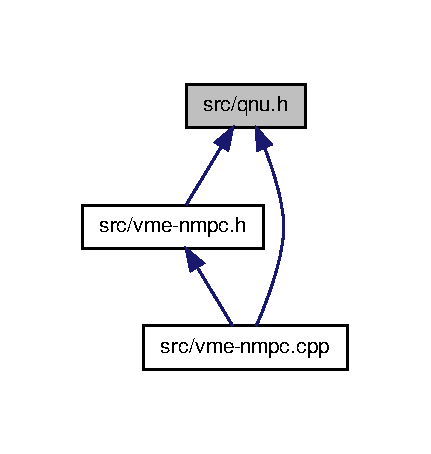
\includegraphics[width=207pt]{qnu_8h__dep__incl}
\end{center}
\end{figure}
\subsection*{Classes}
\begin{DoxyCompactItemize}
\item 
struct \hyperlink{structqnutag}{qnutag}
\item 
struct \hyperlink{struct_lagrtag}{Lagrtag}
\end{DoxyCompactItemize}
\subsection*{Typedefs}
\begin{DoxyCompactItemize}
\item 
typedef struct \hyperlink{structqnutag}{qnutag} \hyperlink{qnu_8h_a3b05f1f30c55bb80f8a3d3b63ad822db}{qnu}
\item 
typedef struct \hyperlink{struct_lagrtag}{Lagrtag} \hyperlink{qnu_8h_a0a3e54bd51fcd867a223ae23fd3c545f}{Lagr}
\end{DoxyCompactItemize}


\subsection{Typedef Documentation}
\hypertarget{qnu_8h_a0a3e54bd51fcd867a223ae23fd3c545f}{\index{qnu.\-h@{qnu.\-h}!Lagr@{Lagr}}
\index{Lagr@{Lagr}!qnu.h@{qnu.\-h}}
\subsubsection[{Lagr}]{\setlength{\rightskip}{0pt plus 5cm}typedef struct {\bf Lagrtag}  {\bf Lagr}}}\label{qnu_8h_a0a3e54bd51fcd867a223ae23fd3c545f}
The Lagr holds the langrange multipliers and related variables. An array of these holds the lagrange multipliers for the N\-M\-P\-C horizon. \hypertarget{qnu_8h_a3b05f1f30c55bb80f8a3d3b63ad822db}{\index{qnu.\-h@{qnu.\-h}!qnu@{qnu}}
\index{qnu@{qnu}!qnu.h@{qnu.\-h}}
\subsubsection[{qnu}]{\setlength{\rightskip}{0pt plus 5cm}typedef struct {\bf qnutag}  {\bf qnu}}}\label{qnu_8h_a3b05f1f30c55bb80f8a3d3b63ad822db}
The qnu structure holds q and u related variables for the robot. An array of qnu holds the state and conrol information for the N\-M\-P\-C horizon. 
\hypertarget{robot_8cpp}{\section{src/robot.cpp File Reference}
\label{robot_8cpp}\index{src/robot.\-cpp@{src/robot.\-cpp}}
}
{\ttfamily \#include \char`\"{}robot.\-h\char`\"{}}\\*
{\ttfamily \#include $<$stdio.\-h$>$}\\*
{\ttfamily \#include $<$stdlib.\-h$>$}\\*
{\ttfamily \#include $<$unistd.\-h$>$}\\*
{\ttfamily \#include $<$string.\-h$>$}\\*
{\ttfamily \#include $<$sys/types.\-h$>$}\\*
{\ttfamily \#include $<$sys/socket.\-h$>$}\\*
{\ttfamily \#include $<$netinet/in.\-h$>$}\\*
{\ttfamily \#include $<$netdb.\-h$>$}\\*
{\ttfamily \#include \char`\"{}errinclude.\-h\char`\"{}}\\*
Include dependency graph for robot.\-cpp\-:
\nopagebreak
\begin{figure}[H]
\begin{center}
\leavevmode
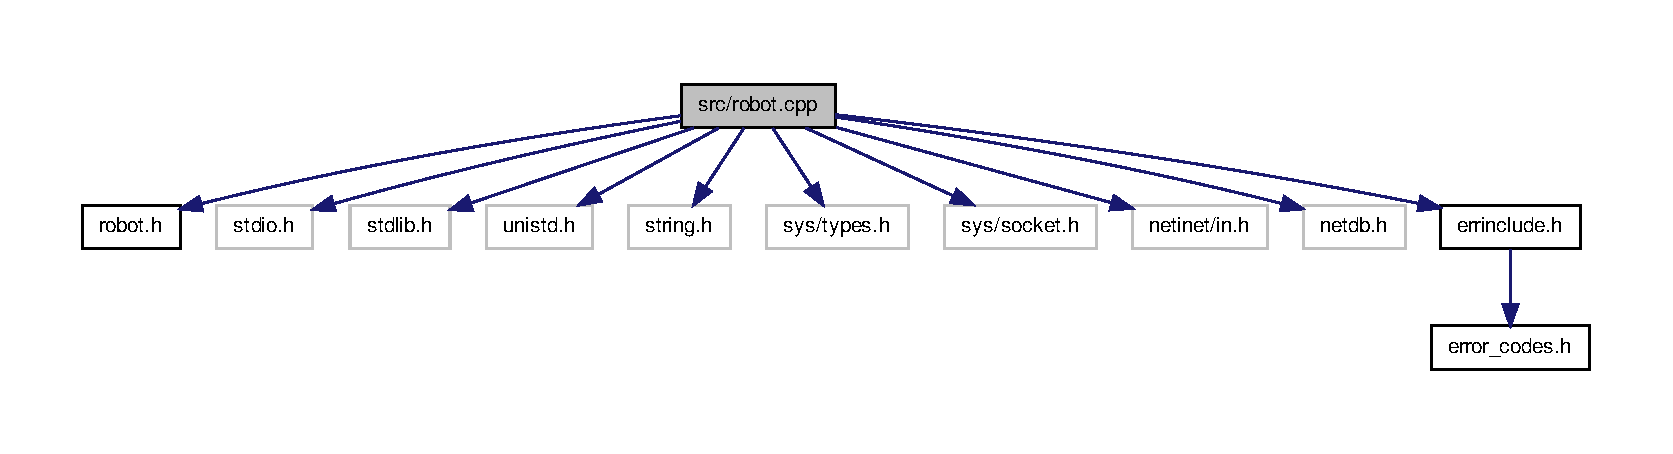
\includegraphics[width=350pt]{robot_8cpp__incl}
\end{center}
\end{figure}

\hypertarget{robot_8h}{\section{src/robot.h File Reference}
\label{robot_8h}\index{src/robot.\-h@{src/robot.\-h}}
}
This graph shows which files directly or indirectly include this file\-:
\nopagebreak
\begin{figure}[H]
\begin{center}
\leavevmode
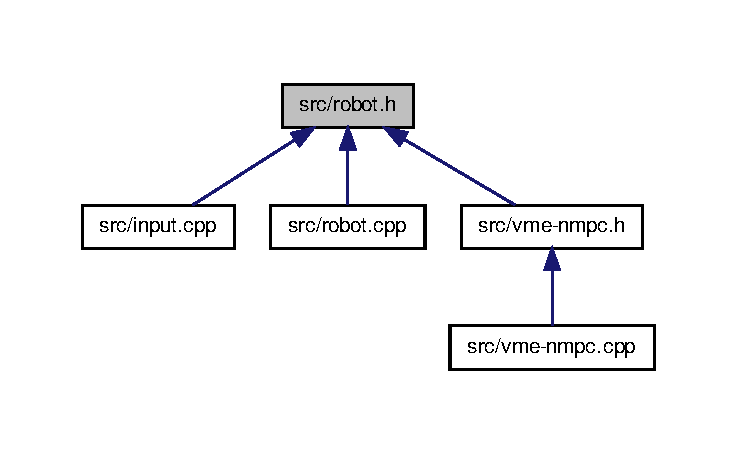
\includegraphics[width=350pt]{robot_8h__dep__incl}
\end{center}
\end{figure}
\subsection*{Classes}
\begin{DoxyCompactItemize}
\item 
class \hyperlink{classrobot}{robot}
\end{DoxyCompactItemize}

\hypertarget{vme-nmpc_8cpp}{\section{src/vme-\/nmpc.cpp File Reference}
\label{vme-nmpc_8cpp}\index{src/vme-\/nmpc.\-cpp@{src/vme-\/nmpc.\-cpp}}
}
{\ttfamily \#include $<$stdio.\-h$>$}\\*
{\ttfamily \#include $<$math.\-h$>$}\\*
{\ttfamily \#include $<$stdlib.\-h$>$}\\*
{\ttfamily \#include $<$unistd.\-h$>$}\\*
{\ttfamily \#include $<$time.\-h$>$}\\*
{\ttfamily \#include \char`\"{}vme-\/nmpc.\-h\char`\"{}}\\*
{\ttfamily \#include \char`\"{}qnu.\-h\char`\"{}}\\*
Include dependency graph for vme-\/nmpc.cpp\-:
\nopagebreak
\begin{figure}[H]
\begin{center}
\leavevmode
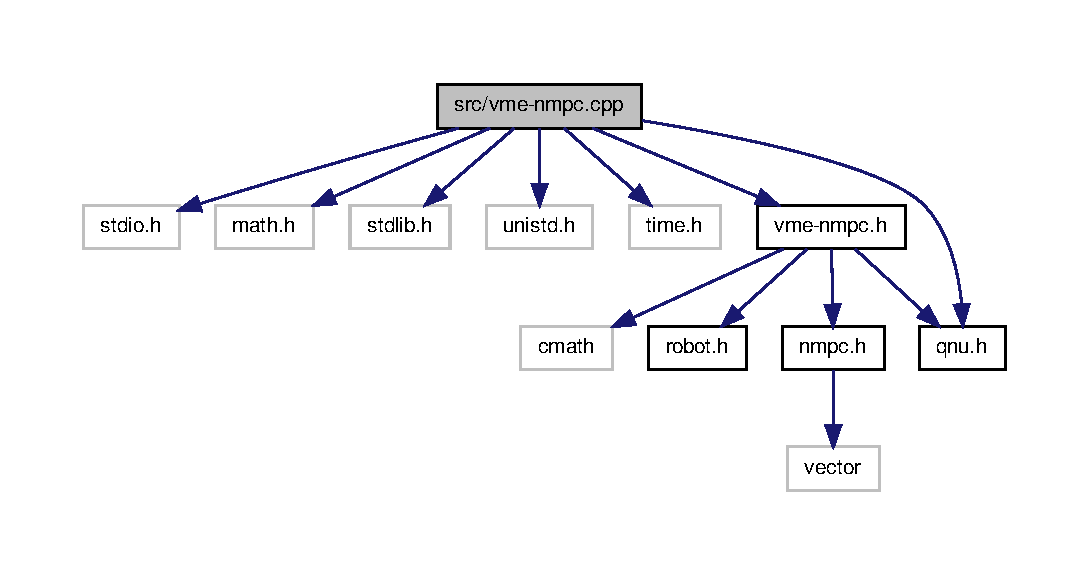
\includegraphics[width=350pt]{vme-nmpc_8cpp__incl}
\end{center}
\end{figure}
\subsection*{Macros}
\begin{DoxyCompactItemize}
\item 
\#define \hyperlink{vme-nmpc_8cpp_a3b04f7ae919ef7628774db8d24ee2c6d}{S\-E\-C\-\_\-\-T\-O\-\_\-\-U\-S\-E\-C}~1\-E+6
\end{DoxyCompactItemize}
\subsection*{Functions}
\begin{DoxyCompactItemize}
\item 
int \hyperlink{vme-nmpc_8cpp_a3c04138a5bfe5d72780bb7e82a18e627}{main} (int argc, char $\ast$$\ast$argv)
\end{DoxyCompactItemize}


\subsection{Macro Definition Documentation}
\hypertarget{vme-nmpc_8cpp_a3b04f7ae919ef7628774db8d24ee2c6d}{\index{vme-\/nmpc.\-cpp@{vme-\/nmpc.\-cpp}!S\-E\-C\-\_\-\-T\-O\-\_\-\-U\-S\-E\-C@{S\-E\-C\-\_\-\-T\-O\-\_\-\-U\-S\-E\-C}}
\index{S\-E\-C\-\_\-\-T\-O\-\_\-\-U\-S\-E\-C@{S\-E\-C\-\_\-\-T\-O\-\_\-\-U\-S\-E\-C}!vme-nmpc.cpp@{vme-\/nmpc.\-cpp}}
\subsubsection[{S\-E\-C\-\_\-\-T\-O\-\_\-\-U\-S\-E\-C}]{\setlength{\rightskip}{0pt plus 5cm}\#define S\-E\-C\-\_\-\-T\-O\-\_\-\-U\-S\-E\-C~1\-E+6}}\label{vme-nmpc_8cpp_a3b04f7ae919ef7628774db8d24ee2c6d}


Definition at line 33 of file vme-\/nmpc.\-cpp.



\subsection{Function Documentation}
\hypertarget{vme-nmpc_8cpp_a3c04138a5bfe5d72780bb7e82a18e627}{\index{vme-\/nmpc.\-cpp@{vme-\/nmpc.\-cpp}!main@{main}}
\index{main@{main}!vme-nmpc.cpp@{vme-\/nmpc.\-cpp}}
\subsubsection[{main}]{\setlength{\rightskip}{0pt plus 5cm}int main (
\begin{DoxyParamCaption}
\item[{int}]{argc, }
\item[{char $\ast$$\ast$}]{argv}
\end{DoxyParamCaption}
)}}\label{vme-nmpc_8cpp_a3c04138a5bfe5d72780bb7e82a18e627}


Definition at line 35 of file vme-\/nmpc.\-cpp.



Here is the call graph for this function\-:
\nopagebreak
\begin{figure}[H]
\begin{center}
\leavevmode
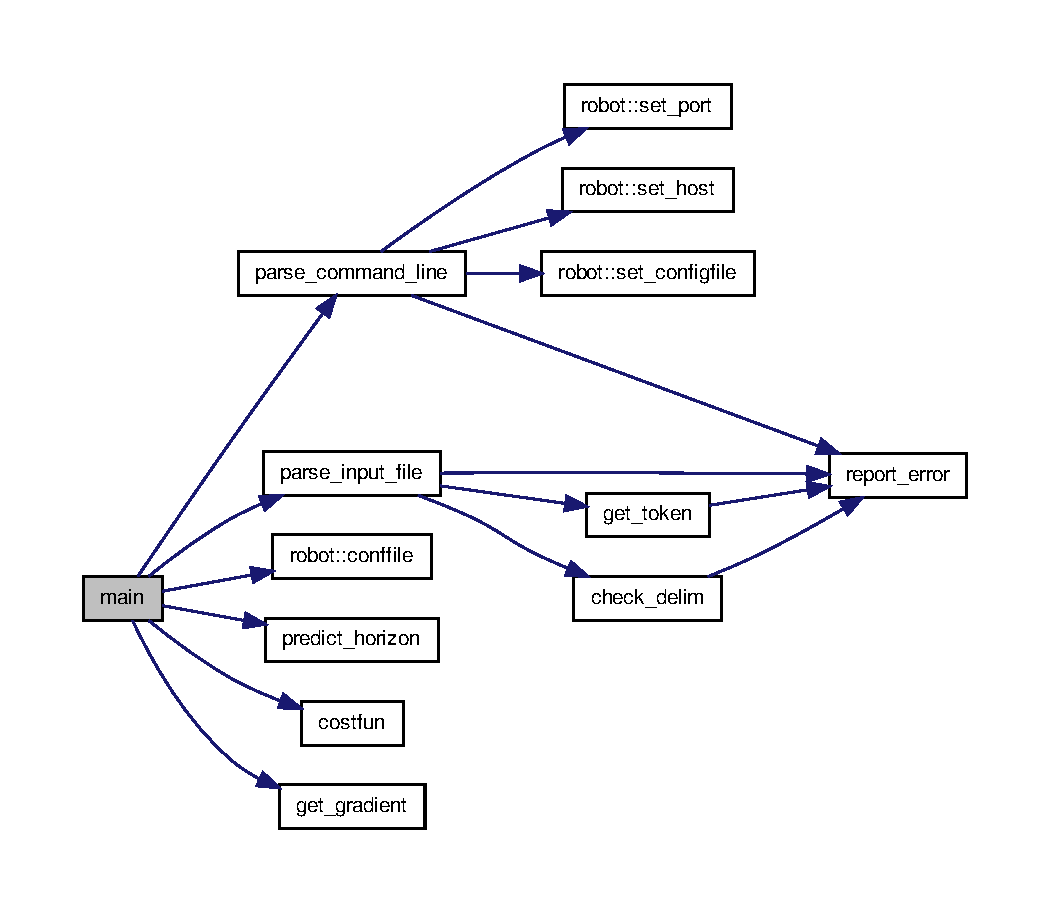
\includegraphics[width=350pt]{vme-nmpc_8cpp_a3c04138a5bfe5d72780bb7e82a18e627_cgraph}
\end{center}
\end{figure}



\hypertarget{vme-nmpc_8h}{\section{src/vme-\/nmpc.h File Reference}
\label{vme-nmpc_8h}\index{src/vme-\/nmpc.\-h@{src/vme-\/nmpc.\-h}}
}
{\ttfamily \#include $<$cmath$>$}\\*
{\ttfamily \#include \char`\"{}robot.\-h\char`\"{}}\\*
{\ttfamily \#include \char`\"{}nmpc.\-h\char`\"{}}\\*
{\ttfamily \#include \char`\"{}qnu.\-h\char`\"{}}\\*
Include dependency graph for vme-\/nmpc.h\-:
\nopagebreak
\begin{figure}[H]
\begin{center}
\leavevmode
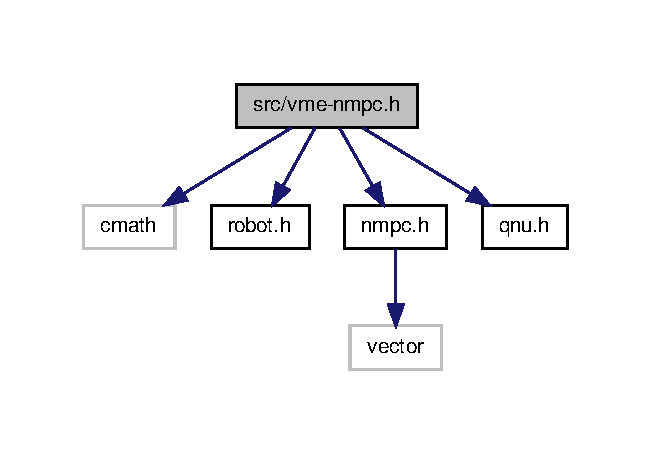
\includegraphics[width=312pt]{vme-nmpc_8h__incl}
\end{center}
\end{figure}
This graph shows which files directly or indirectly include this file\-:
\nopagebreak
\begin{figure}[H]
\begin{center}
\leavevmode
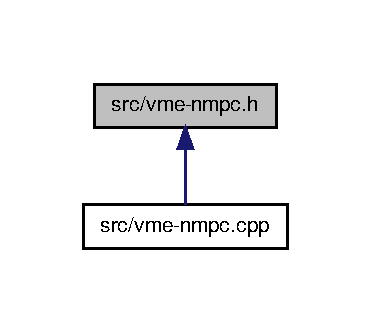
\includegraphics[width=178pt]{vme-nmpc_8h__dep__incl}
\end{center}
\end{figure}
\subsection*{Functions}
\begin{DoxyCompactItemize}
\item 
int \hyperlink{vme-nmpc_8h_ae023f8cf4938bafee258ec79c83f5e7d}{init\-\_\-vme\-\_\-sock} ()
\item 
int \hyperlink{vme-nmpc_8h_a383fbb6b26fb0e0638ab4816c0037c0e}{parse\-\_\-command\-\_\-line} (int, char $\ast$$\ast$, \hyperlink{classrobot}{robot} $\ast$)
\item 
void \hyperlink{vme-nmpc_8h_a08b905d7f390613ae37c835938f13207}{parse\-\_\-input\-\_\-file} (\hyperlink{nmpc_8h_a071459b3a1fa3748660f7de5d6ab38d0}{nmpc} \&, const char $\ast$)
\item 
float \hyperlink{vme-nmpc_8h_aa075c06c19ff3b551ff1f9ddff3d2181}{costfun} (const \hyperlink{qnu_8h_a3b05f1f30c55bb80f8a3d3b63ad822db}{qnu} $\ast$qu, const \hyperlink{qnu_8h_a0a3e54bd51fcd867a223ae23fd3c545f}{Lagr} $\ast$p, const \hyperlink{nmpc_8h_a071459b3a1fa3748660f7de5d6ab38d0}{nmpc} \&C)
\item 
void \hyperlink{vme-nmpc_8h_a293565f06dcf7e375ac1b53f3b9b0a0b}{predict\-\_\-horizon} (\hyperlink{qnu_8h_a3b05f1f30c55bb80f8a3d3b63ad822db}{qnu} $\ast$qu, \hyperlink{qnu_8h_a0a3e54bd51fcd867a223ae23fd3c545f}{Lagr} $\ast$p, const \hyperlink{nmpc_8h_a071459b3a1fa3748660f7de5d6ab38d0}{nmpc} \&C)
\item 
void \hyperlink{vme-nmpc_8h_a6db4a98664c521bc4d1f3e768672ddc8}{get\-\_\-gradient} (\hyperlink{qnu_8h_a3b05f1f30c55bb80f8a3d3b63ad822db}{qnu} $\ast$qu, \hyperlink{qnu_8h_a0a3e54bd51fcd867a223ae23fd3c545f}{Lagr} $\ast$p, \hyperlink{nmpc_8h_a071459b3a1fa3748660f7de5d6ab38d0}{nmpc} \&C, float $\ast$grad)
\end{DoxyCompactItemize}


\subsection{Function Documentation}
\hypertarget{vme-nmpc_8h_aa075c06c19ff3b551ff1f9ddff3d2181}{\index{vme-\/nmpc.\-h@{vme-\/nmpc.\-h}!costfun@{costfun}}
\index{costfun@{costfun}!vme-nmpc.h@{vme-\/nmpc.\-h}}
\subsubsection[{costfun}]{\setlength{\rightskip}{0pt plus 5cm}float costfun (
\begin{DoxyParamCaption}
\item[{const {\bf qnu} $\ast$}]{qu, }
\item[{const {\bf Lagr} $\ast$}]{p, }
\item[{const {\bf nmpc} \&}]{C}
\end{DoxyParamCaption}
)\hspace{0.3cm}{\ttfamily [inline]}}}\label{vme-nmpc_8h_aa075c06c19ff3b551ff1f9ddff3d2181}


Definition at line 37 of file vme-\/nmpc.\-h.



Here is the caller graph for this function\-:
\nopagebreak
\begin{figure}[H]
\begin{center}
\leavevmode
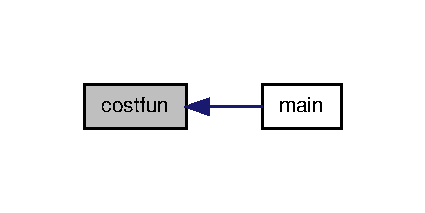
\includegraphics[width=204pt]{vme-nmpc_8h_aa075c06c19ff3b551ff1f9ddff3d2181_icgraph}
\end{center}
\end{figure}


\hypertarget{vme-nmpc_8h_a6db4a98664c521bc4d1f3e768672ddc8}{\index{vme-\/nmpc.\-h@{vme-\/nmpc.\-h}!get\-\_\-gradient@{get\-\_\-gradient}}
\index{get\-\_\-gradient@{get\-\_\-gradient}!vme-nmpc.h@{vme-\/nmpc.\-h}}
\subsubsection[{get\-\_\-gradient}]{\setlength{\rightskip}{0pt plus 5cm}void get\-\_\-gradient (
\begin{DoxyParamCaption}
\item[{{\bf qnu} $\ast$}]{qu, }
\item[{{\bf Lagr} $\ast$}]{p, }
\item[{{\bf nmpc} \&}]{C, }
\item[{float $\ast$}]{grad}
\end{DoxyParamCaption}
)\hspace{0.3cm}{\ttfamily [inline]}}}\label{vme-nmpc_8h_a6db4a98664c521bc4d1f3e768672ddc8}
Calculate gradient from ∂\-J = ∑∂\-H/∂u ∂u, then step the control set. To get the gradient ∂\-H/∂u\-\_\-k, for each step, k in the horizon, loop through each k in N. This involves computing the obstacle potential and Lagrange multipliers. Then, the control plan is updated by stepping against the direction of the gradient.

Compute the obstacle potential by looping through the list of obstacles\-:

F\-I\-X\-M\-E\-: Probably best to remove the vectors from C and use arrays. Vectors could be used temporarily to expand the data from the input file to memory. Error checking for the number of coordinates can be done there.

Definition at line 90 of file vme-\/nmpc.\-h.



Here is the caller graph for this function\-:
\nopagebreak
\begin{figure}[H]
\begin{center}
\leavevmode
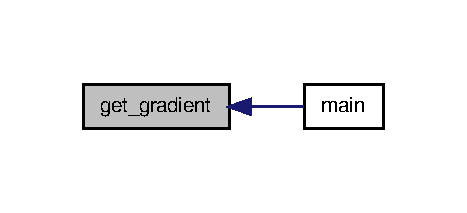
\includegraphics[width=224pt]{vme-nmpc_8h_a6db4a98664c521bc4d1f3e768672ddc8_icgraph}
\end{center}
\end{figure}


\hypertarget{vme-nmpc_8h_ae023f8cf4938bafee258ec79c83f5e7d}{\index{vme-\/nmpc.\-h@{vme-\/nmpc.\-h}!init\-\_\-vme\-\_\-sock@{init\-\_\-vme\-\_\-sock}}
\index{init\-\_\-vme\-\_\-sock@{init\-\_\-vme\-\_\-sock}!vme-nmpc.h@{vme-\/nmpc.\-h}}
\subsubsection[{init\-\_\-vme\-\_\-sock}]{\setlength{\rightskip}{0pt plus 5cm}int init\-\_\-vme\-\_\-sock (
\begin{DoxyParamCaption}
{}
\end{DoxyParamCaption}
)}}\label{vme-nmpc_8h_ae023f8cf4938bafee258ec79c83f5e7d}
\hypertarget{vme-nmpc_8h_a383fbb6b26fb0e0638ab4816c0037c0e}{\index{vme-\/nmpc.\-h@{vme-\/nmpc.\-h}!parse\-\_\-command\-\_\-line@{parse\-\_\-command\-\_\-line}}
\index{parse\-\_\-command\-\_\-line@{parse\-\_\-command\-\_\-line}!vme-nmpc.h@{vme-\/nmpc.\-h}}
\subsubsection[{parse\-\_\-command\-\_\-line}]{\setlength{\rightskip}{0pt plus 5cm}int parse\-\_\-command\-\_\-line (
\begin{DoxyParamCaption}
\item[{int}]{, }
\item[{char $\ast$$\ast$}]{, }
\item[{{\bf robot} $\ast$}]{}
\end{DoxyParamCaption}
)}}\label{vme-nmpc_8h_a383fbb6b26fb0e0638ab4816c0037c0e}


Definition at line 32 of file input.\-cpp.



Here is the call graph for this function\-:
\nopagebreak
\begin{figure}[H]
\begin{center}
\leavevmode
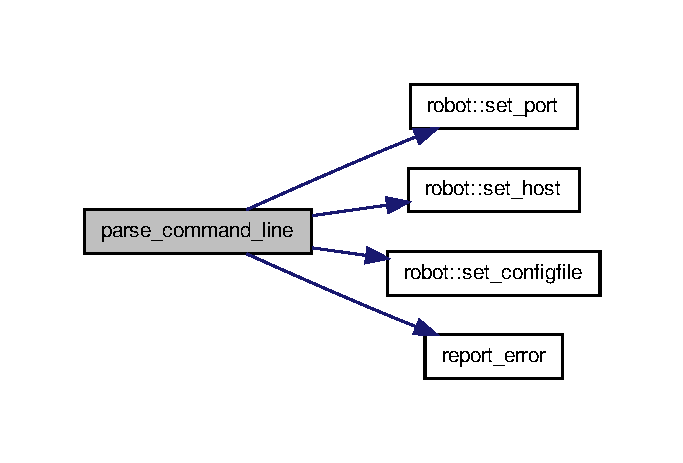
\includegraphics[width=328pt]{vme-nmpc_8h_a383fbb6b26fb0e0638ab4816c0037c0e_cgraph}
\end{center}
\end{figure}




Here is the caller graph for this function\-:
\nopagebreak
\begin{figure}[H]
\begin{center}
\leavevmode
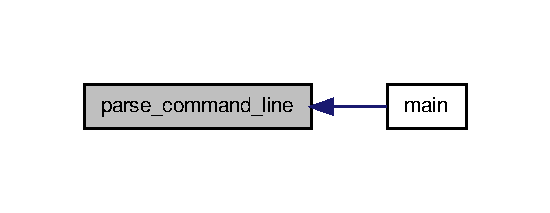
\includegraphics[width=264pt]{vme-nmpc_8h_a383fbb6b26fb0e0638ab4816c0037c0e_icgraph}
\end{center}
\end{figure}


\hypertarget{vme-nmpc_8h_a08b905d7f390613ae37c835938f13207}{\index{vme-\/nmpc.\-h@{vme-\/nmpc.\-h}!parse\-\_\-input\-\_\-file@{parse\-\_\-input\-\_\-file}}
\index{parse\-\_\-input\-\_\-file@{parse\-\_\-input\-\_\-file}!vme-nmpc.h@{vme-\/nmpc.\-h}}
\subsubsection[{parse\-\_\-input\-\_\-file}]{\setlength{\rightskip}{0pt plus 5cm}void parse\-\_\-input\-\_\-file (
\begin{DoxyParamCaption}
\item[{{\bf nmpc} \&}]{, }
\item[{const char $\ast$}]{}
\end{DoxyParamCaption}
)}}\label{vme-nmpc_8h_a08b905d7f390613ae37c835938f13207}


Definition at line 215 of file input.\-cpp.



Here is the call graph for this function\-:
\nopagebreak
\begin{figure}[H]
\begin{center}
\leavevmode
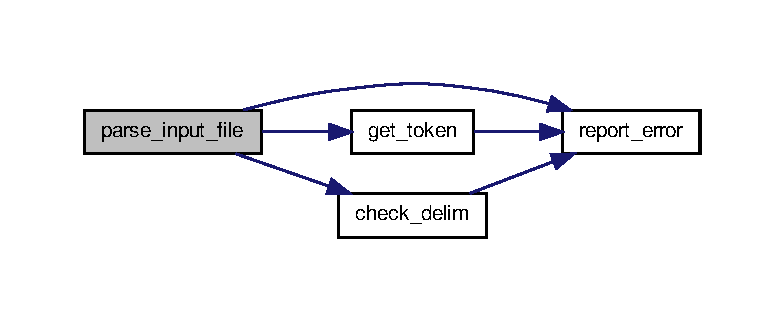
\includegraphics[width=350pt]{vme-nmpc_8h_a08b905d7f390613ae37c835938f13207_cgraph}
\end{center}
\end{figure}




Here is the caller graph for this function\-:
\nopagebreak
\begin{figure}[H]
\begin{center}
\leavevmode
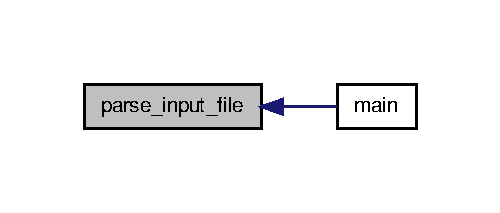
\includegraphics[width=240pt]{vme-nmpc_8h_a08b905d7f390613ae37c835938f13207_icgraph}
\end{center}
\end{figure}


\hypertarget{vme-nmpc_8h_a293565f06dcf7e375ac1b53f3b9b0a0b}{\index{vme-\/nmpc.\-h@{vme-\/nmpc.\-h}!predict\-\_\-horizon@{predict\-\_\-horizon}}
\index{predict\-\_\-horizon@{predict\-\_\-horizon}!vme-nmpc.h@{vme-\/nmpc.\-h}}
\subsubsection[{predict\-\_\-horizon}]{\setlength{\rightskip}{0pt plus 5cm}void predict\-\_\-horizon (
\begin{DoxyParamCaption}
\item[{{\bf qnu} $\ast$}]{qu, }
\item[{{\bf Lagr} $\ast$}]{p, }
\item[{const {\bf nmpc} \&}]{C}
\end{DoxyParamCaption}
)\hspace{0.3cm}{\ttfamily [inline]}}}\label{vme-nmpc_8h_a293565f06dcf7e375ac1b53f3b9b0a0b}
This function approximates the state trajectory of the system b ased on a set of control input. It is used to optimize the control input by giving an approximate path to build an approximation of the cost measure of possible movements. For all times in the horizon, provide an approximation of the state vector, based on a simple Euler integration scheme.

Definition at line 61 of file vme-\/nmpc.\-h.



Here is the caller graph for this function\-:
\nopagebreak
\begin{figure}[H]
\begin{center}
\leavevmode
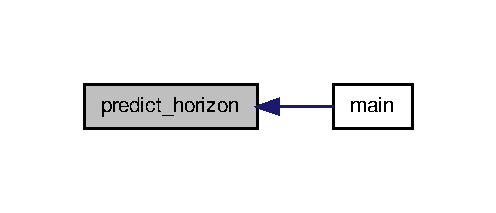
\includegraphics[width=238pt]{vme-nmpc_8h_a293565f06dcf7e375ac1b53f3b9b0a0b_icgraph}
\end{center}
\end{figure}



\addcontentsline{toc}{part}{Index}
\printindex
\end{document}
